\documentclass[UTF8]{ctexart}

\usepackage{amsmath}
\usepackage{amssymb}
\usepackage{mathrsfs}
\usepackage{bm}
\usepackage{hyperref}
\usepackage{multirow}
\usepackage{multicol}
\usepackage{diagbox}
\usepackage{tabularx}
\usepackage{booktabs}
\usepackage{longtable}
\usepackage{float}
\usepackage{array}
\usepackage{pifont}
\usepackage{ulem}
\usepackage{cases}
\usepackage{cite}
\usepackage{graphicx}
\usepackage[margin=1in]{geometry}
\usepackage{fancyhdr}
\usepackage{float}
\usepackage{listings}
\usepackage{xcolor}
\usepackage{fontspec}
\setmainfont{Arial}
\usepackage{titling}
\pagestyle{fancy}
\fancyhf{}
\geometry{a4paper}

\setlength{\headheight}{29.87538pt}
\addtolength{\topmargin}{-17.87538pt}

\lstset{ %代码块设置
    language = C,
    numbers=left,
    keywordstyle=\color{blue!70},
    commentstyle=\color{red!50!green!50!blue!50},
    frame=shadowbox,
    rulesepcolor=\color{red!20!green!20!blue!20},
    basicstyle=\ttfamily,
    showstringspaces=false
}
\lstset{language=C}

\title{C语言试题}
\author{谭乐闻}
\date{\today}
\pagenumbering{arabic} %设置文章页码为阿拉伯数字

\begin{document}
\fancyhf{}
\fancyhead[L]{ %页眉左侧logo
    \begin{minipage}[c]{0.9\textwidth}
        
\includegraphics[height=10.5mm]{picture/logo1.jpg}
    \end{minipage}
}
\fancyhead[C]{NCUSCC 2024秋招算法考试题}
\fancyfoot[C]{\thepage}

\begin{titlingpage} %封面设置
    \centering
    
\includegraphics[width=0.8\textwidth]{picture/logo2.jpg}

    \vspace{1cm} % Adjust vertical space as needed

    {\Huge \thetitle\par} % Title
    \vspace{1cm}
    {\Large \theauthor\par} % Author
    \vfill
    {\large \thedate\par} % Date
\end{titlingpage}

\newpage

\tableofcontents  %自动根据下文创建目录

\newpage
\section{摘要}
本研究报告详细描述了在虚拟机环境中安装和配置Ubuntu 22.04 LTS操作系统,
并成功安装最新版本的gcc编译器的过程。
报告进一步展示了使用C语言手动实现冒泡排序、基础堆排序和斐波那契堆排序算法,
并通过自编写的测试代码验证了各算法的正确性。为了评估算法的性能,
研究中生成了涵盖不同规模数据集的测试数据,
包括至少100,000条数据的排序任务。
通过使用不同等级的gcc编译优化选项(如-O0, -O1, -O2, -O3, -Ofast),
记录并分析了各优化等级下排序算法的执行时间和资源占用情况。
实验结果以CSV格式记录,并使用Python工具进行了数据可视化,
绘制了矢量图以展示实验结论。报告最终以LaTeX格式撰写,
详细记录了实验环境的搭建、算法实现细节、测试数据生成方法、
性能对比结果以及实验过程中遇到的问题和解决方案。

关键词:虚拟机,Ubuntu 22.04 LTS,gcc编译器,冒泡排序,堆排序,
斐波那契堆排序,编译优化,性能测试,数据可视化。

\section{任务一:安装虚拟机}
\subsection{任务内容}
\begin{itemize}
    \item 在虚拟机中安装 Ubuntu 22.04 LTS 操作系统。
    \item 配置虚拟机的网络连接,确保可以正常联网。
\end{itemize}

\subsection{任务分析}
这条任务的核心是安装虚拟化软件(如 VMware Workstation、Oracle VirtualBox 
或 Parallels Desktop),创建并配置虚拟机,然后在其上安装 Ubuntu 22.04 LTS 
操作系统。安装过程中需要下载 Ubuntu 的 ISO 镜像文件,并将其设置为虚拟机的启动
盘,按照安装向导完成操作系统的安装。随后,配置虚拟机的网络连接,确保其能够
访问外部网络,通常通过设置网络适配器为“桥接模式”或“NAT模式”。最后,更新系统并
安装常用软件,以验证网络连接的正常性。通过这些步骤,用户可以在虚拟环境中成功
运行一个联网的 Ubuntu 系统。

\subsection{任务实现}
\subsubsection{安装虚拟机软件}
\begin{figure}[H]
    \centering
    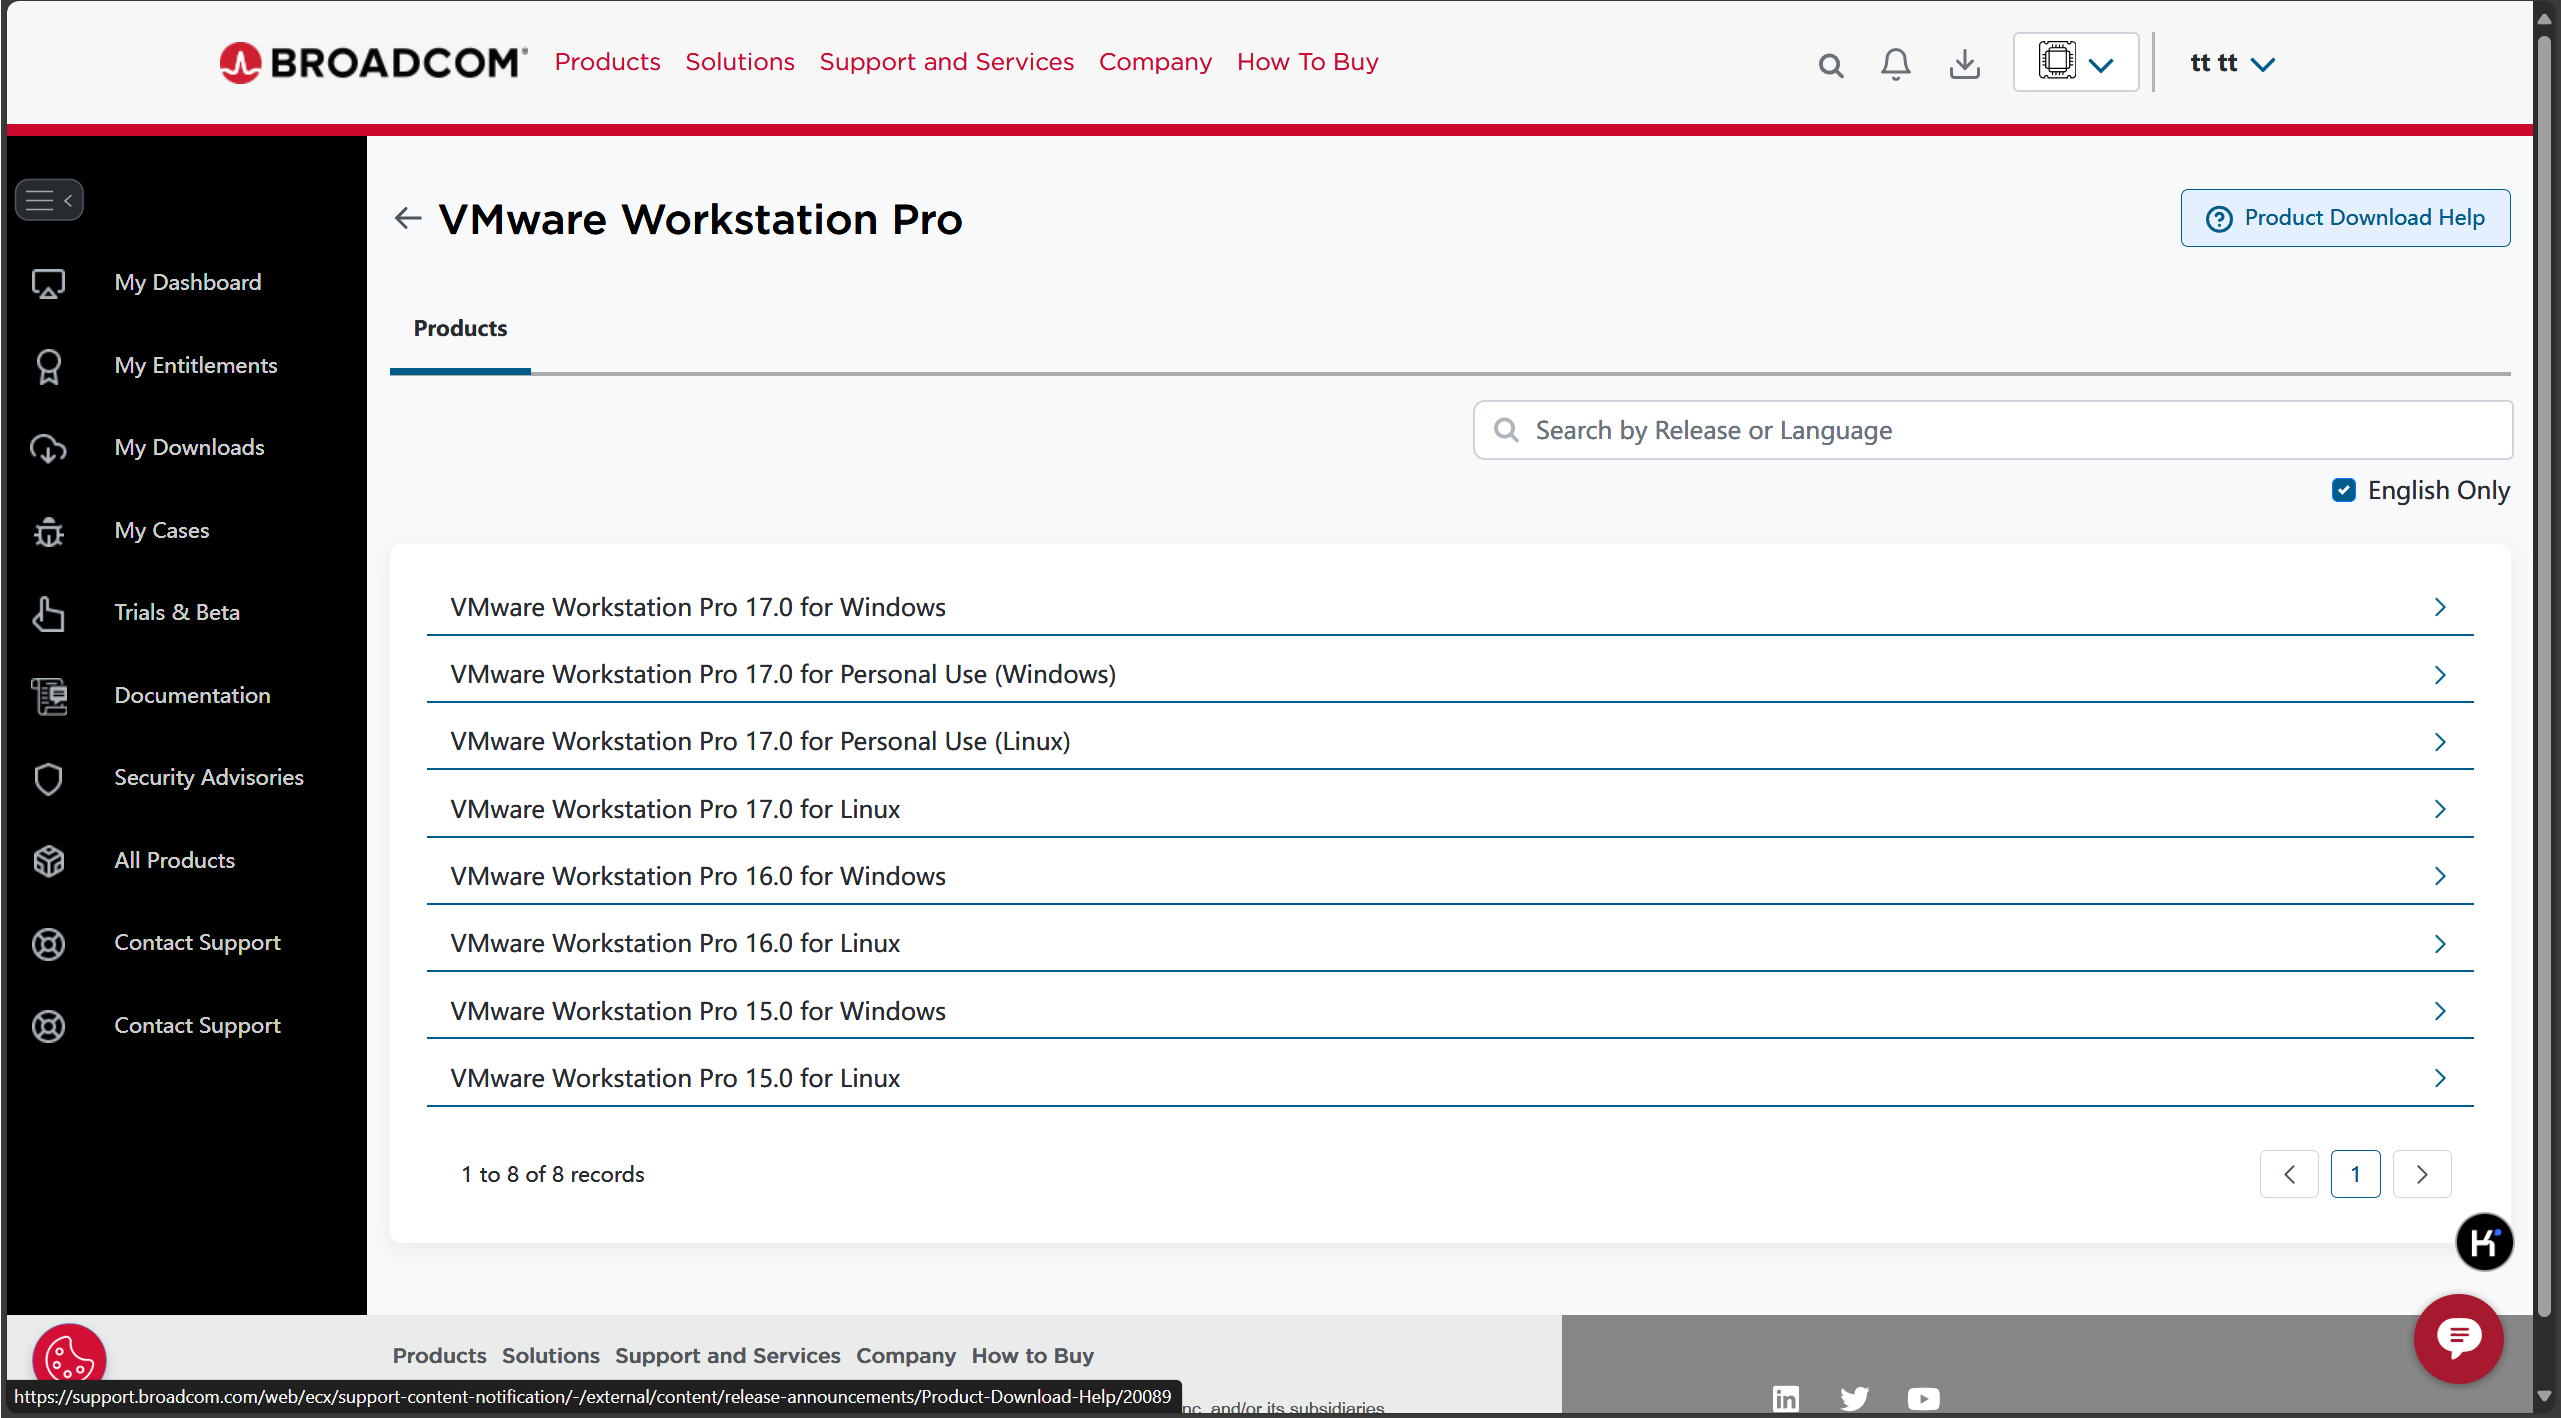
\includegraphics[width=0.95\textwidth]{picture/Screenshot 2024-10-14 095239.png}
    \caption{下载界面}
\end{figure}
首先,需要安装虚拟机软件。本研究使用 VMware Workstation Pro 17.6.1 
作为虚拟机软件。

\begin{figure}[H]
    \centering
    
\includegraphics[width=0.95\textwidth]{picture/Screenshot 2024-10-14 103330.png}
    \caption{安装界面}
\end{figure}
下载完成后,打开安装程序,此界面直接点击“下一步”按钮。

\begin{figure}[H]
    \centering
    
\includegraphics[width=0.95\textwidth]{picture/Screenshot 2024-10-14 103946.png}
    \caption{安装界面}
\end{figure}

勾选“我接受许可协议中的条款”,再点击“下一步”。

\begin{figure}[H]
    \centering
    
\includegraphics[width=0.95\textwidth]{picture/Screenshot 2024-10-14 104456.png}
    \caption{安装界面}
\end{figure}
默认安装位置是“C:/Program Files (x86)/VMware/VMware Workstation/”,点击
旁边的“更改…”按钮可以修改安装路径,我这里修改成“D:/VMware/”。(习惯把软件安装在 D 盘)
\\之后点击“下一步”。

\begin{figure}[H]
    \centering
    
\includegraphics[width=0.95\textwidth]{picture/Screenshot 2024-10-14 105207.png}
    \caption{安装界面}
\end{figure}
此界面把两个选项的勾选全部取消(反正用不到),点击“下一步”。

\begin{figure}[H]
    \centering
    
\includegraphics[width=0.95\textwidth]{picture/Screenshot 2024-10-14 105732.png}
    \caption{安装界面}
\end{figure}
这里我默认全部勾选上,点击“下一步”。

\begin{figure}[H]
    \centering
    
\includegraphics[width=0.95\textwidth]{picture/Screenshot 2024-10-14 105829.png}
    \caption{安装界面}
\end{figure}
点击“安装”即可,大概需要 2 至 3 分钟(由电脑配置而定)。

\begin{figure}[H]
    \centering
    
\includegraphics[width=0.95\textwidth]{picture/Screenshot 2024-10-14 110329.png}
    \caption{安装界面}
\end{figure}
安装完成后,点击“许可证”按钮,在网上找一个许可证填进去。

\begin{figure}[H]
    \centering
    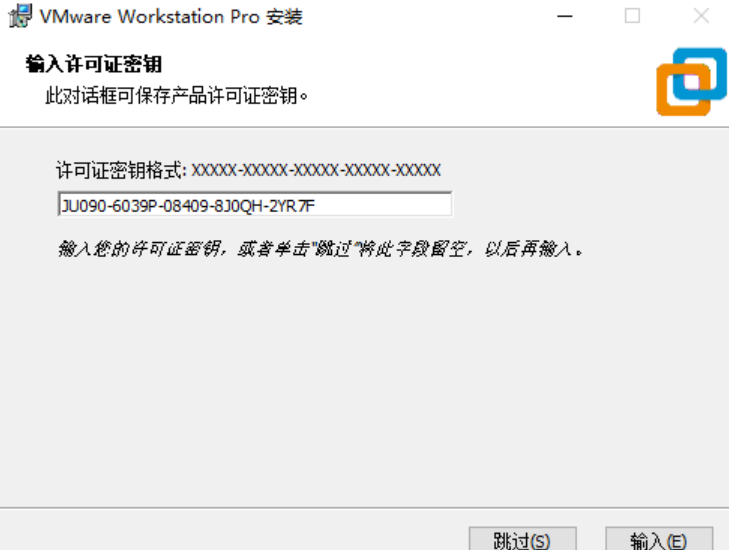
\includegraphics[width=0.95\textwidth]{picture/Screenshot 2024-10-14 110401.png}
    \caption{安装界面}
\end{figure}
把密钥粘贴进来后,点击“输入”按钮。

\begin{figure}[H]
    \centering
    
\includegraphics[width=0.95\textwidth]{picture/Screenshot 2024-10-14 110442.png}
    \caption{安装界面}
\end{figure}
最后单机“完成”按钮,完成安装。

\subsubsection{安装 Ubuntu 22.04 LTS 操作系统}
\begin{figure}[H]
    \centering
    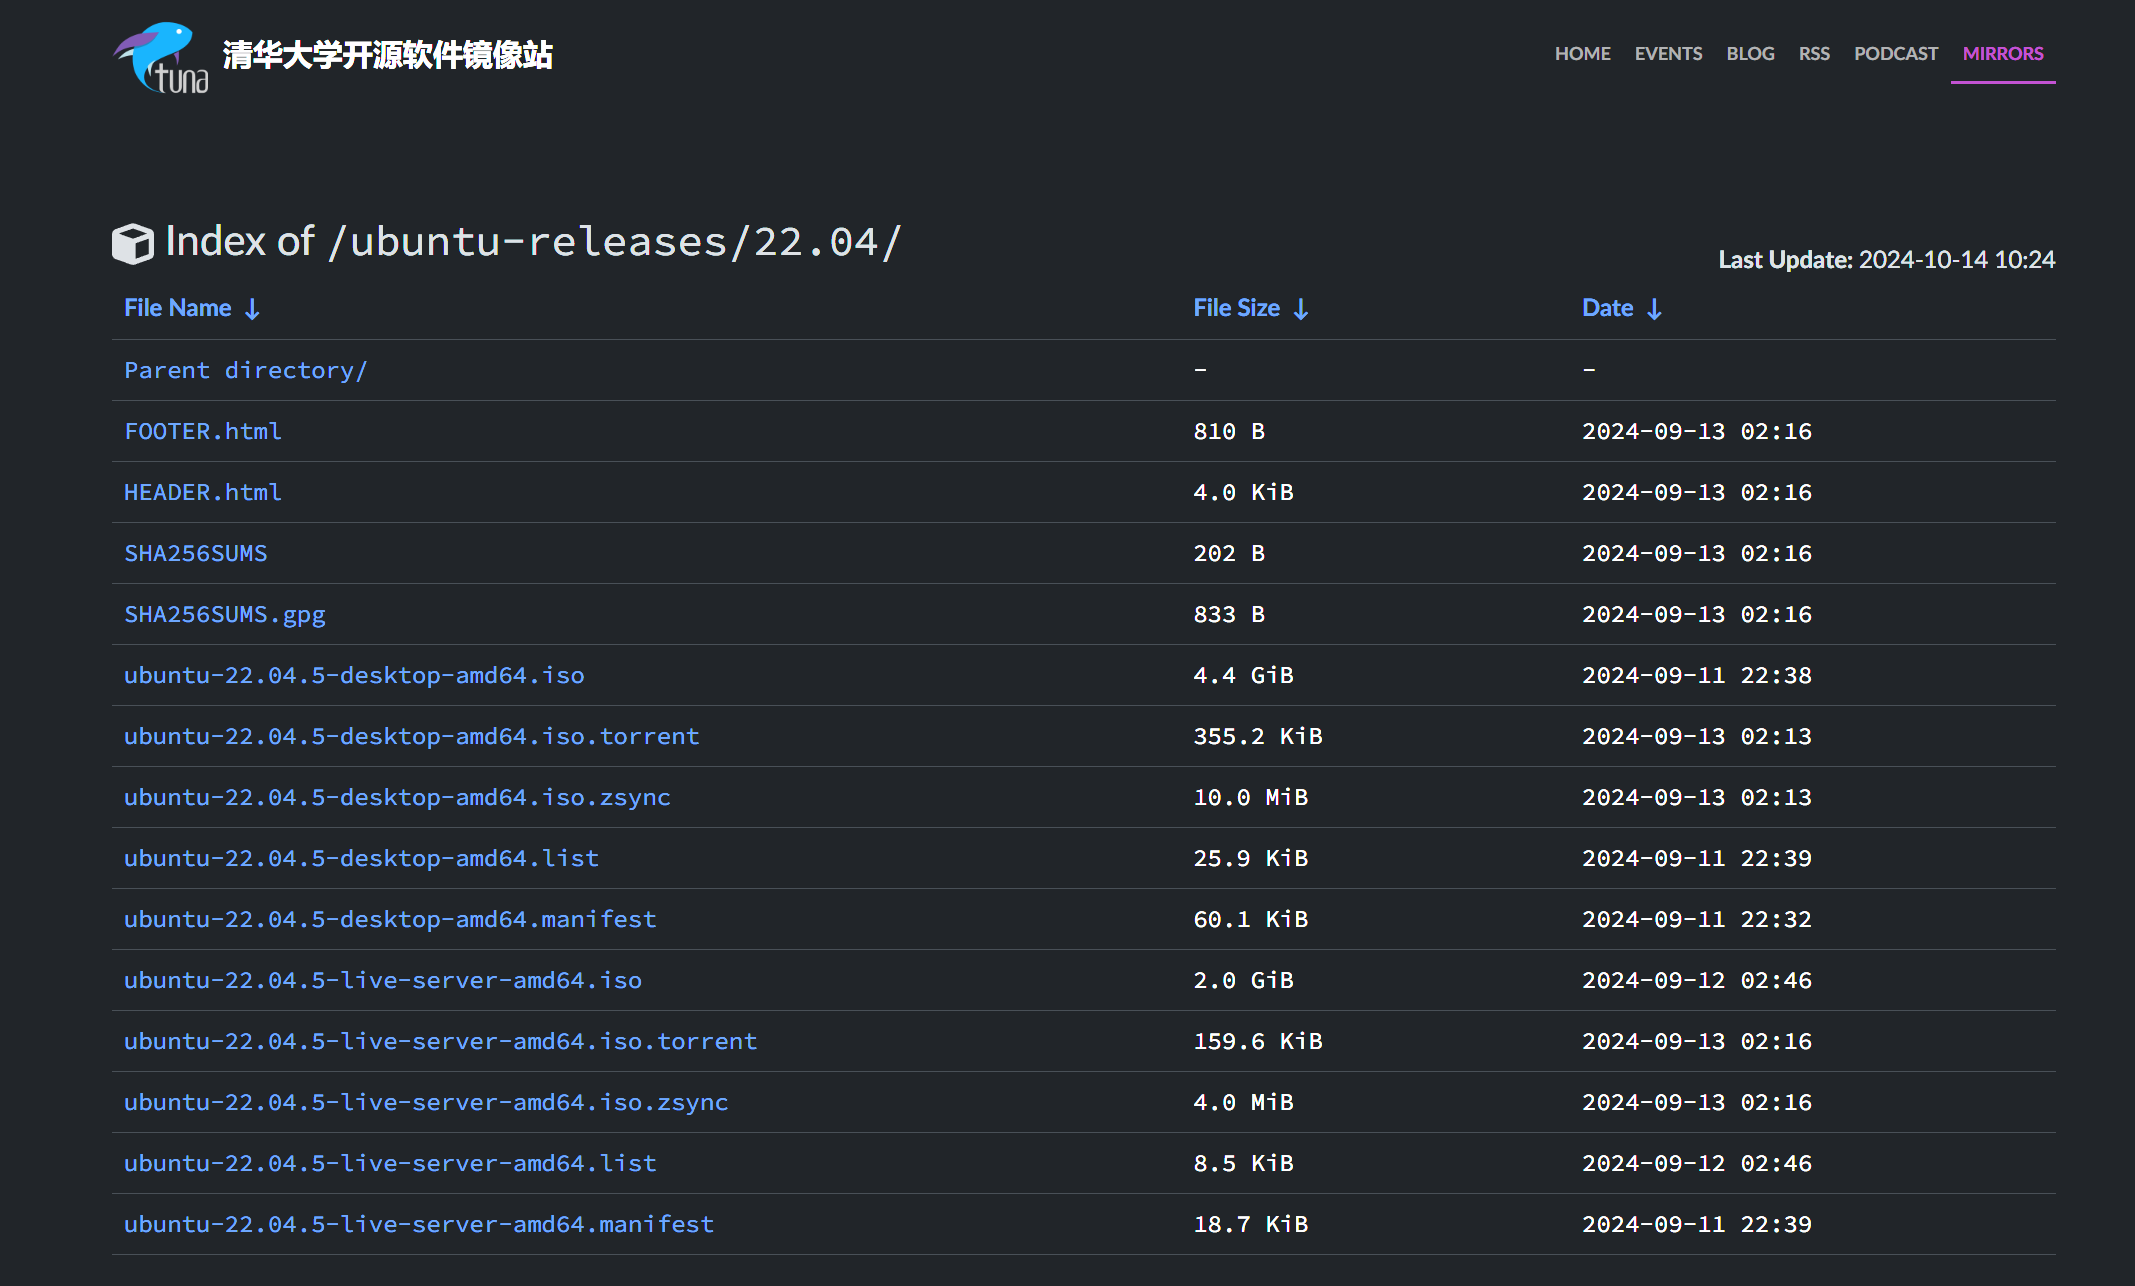
\includegraphics[width=0.95\textwidth]{picture/Screenshot 2024-10-14 111819.png}
    \caption{清华开源镜像站}
\end{figure}
前往清华开源镜像站下载Ubuntu 22.04 LTS amd64镜像

\begin{figure}[H]
    \centering
    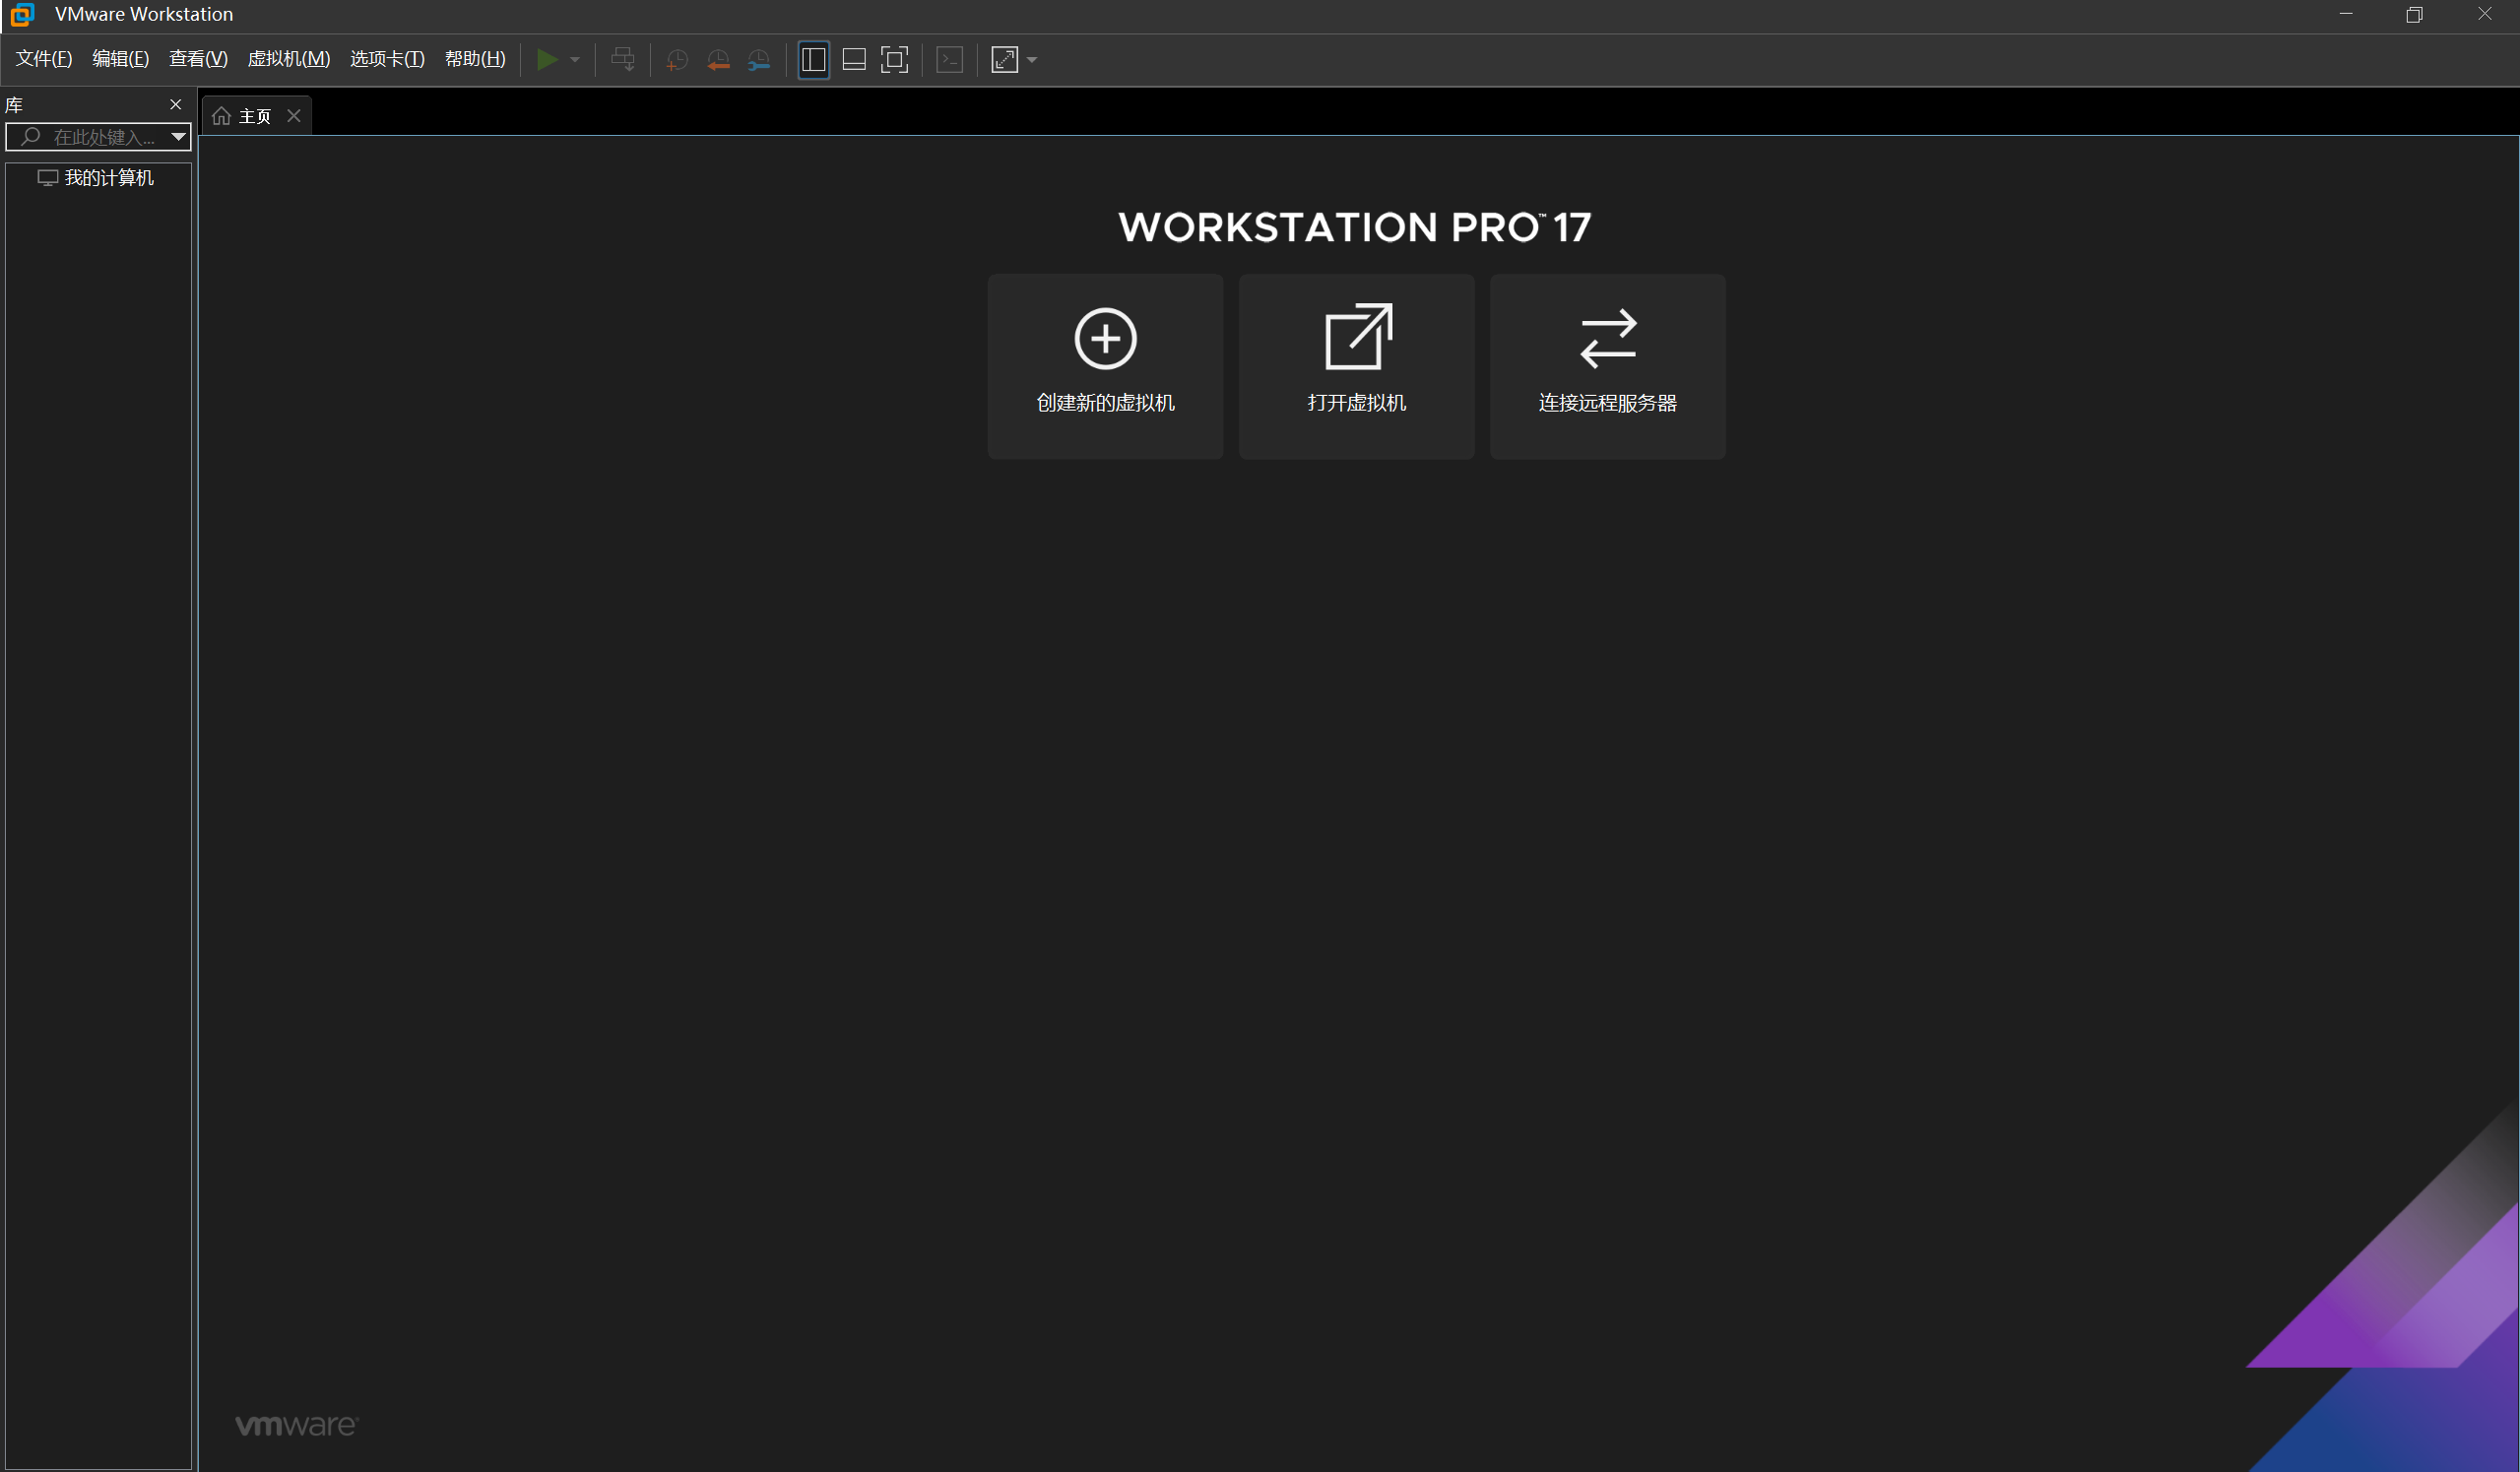
\includegraphics[width=0.95\textwidth]{picture/Screenshot 2024-10-14 112401.png}
    \caption{虚拟机创建界面}
\end{figure}
双击打开刚刚安装好的 VMware Workstation Pro 17,进入软件后,点击“创建新的虚拟机”。

\begin{figure}[H]
    \centering
    
\includegraphics[width=0.95\textwidth]{picture/Screenshot 2024-10-14 112615.png}
    \caption{虚拟机创建界面}
\end{figure}
选择“自定义”选项,点击“下一步”。

\begin{figure}[H]
    \centering
    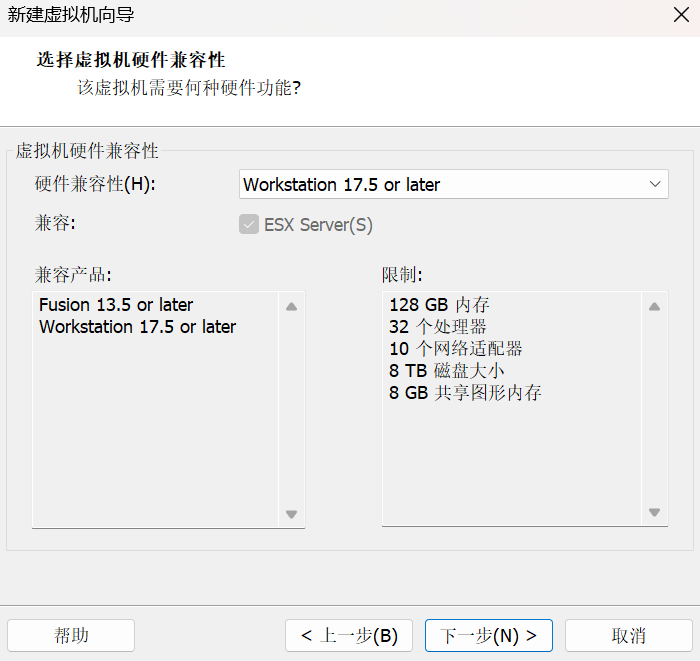
\includegraphics[width=0.95\textwidth]{picture/Screenshot 2024-10-14 112657.png}
    \caption{虚拟机创建界面}
\end{figure}
点击“下一步”。

\begin{figure}[H]
    \centering
    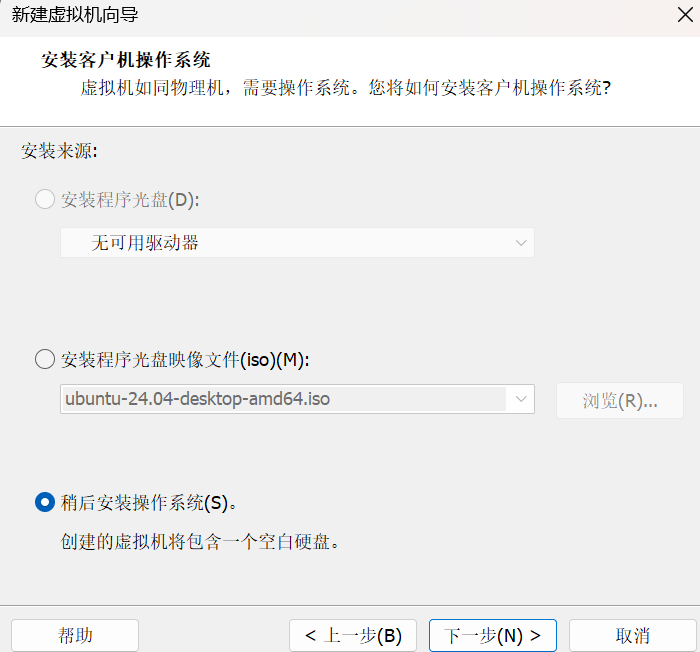
\includegraphics[width=0.95\textwidth]{picture/Screenshot 2024-10-14 112736.png}
    \caption{虚拟机创建界面}
\end{figure}
选择稍后安装操作系统,点击“下一步”。

\begin{figure}[H]
    \centering
    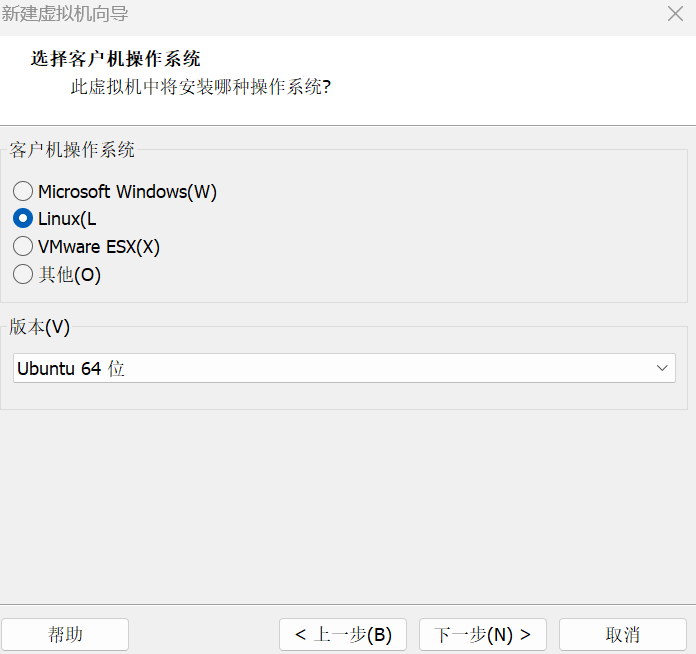
\includegraphics[width=0.95\textwidth]{picture/Screenshot 2024-10-14 112814.png}
    \caption{虚拟机创建界面}
\end{figure}
点击“下一步”。

\begin{figure}[H]
    \centering
    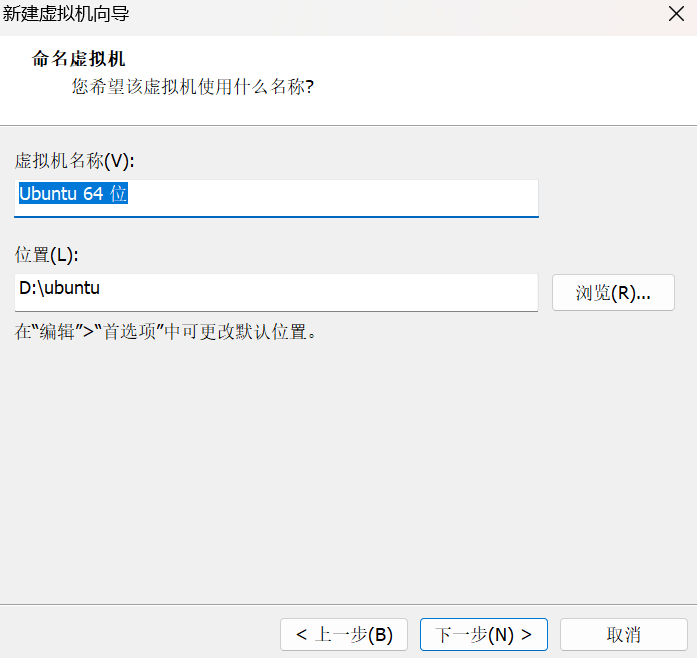
\includegraphics[width=0.95\textwidth]{picture/Screenshot 2024-10-14 113001.png}
    \caption{虚拟机创建界面}
\end{figure}
将安装位置更改为D盘,点击“下一步”。

\begin{figure}[H]
    \centering
    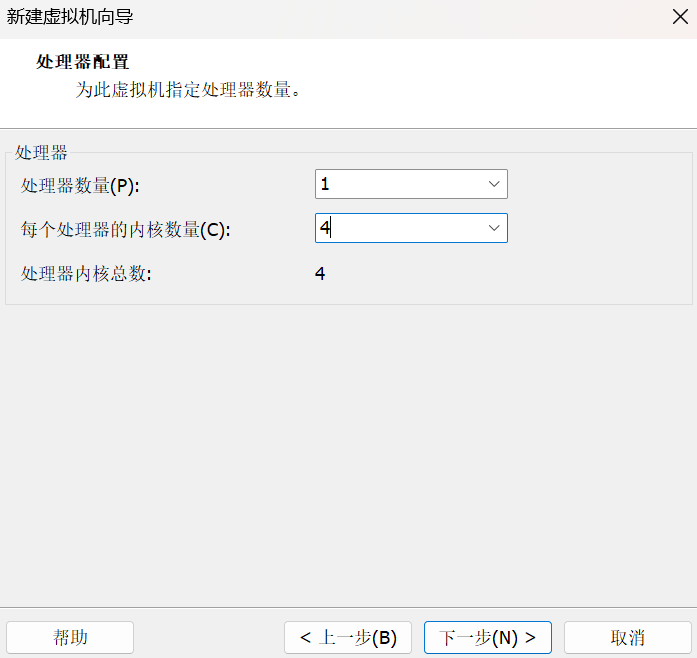
\includegraphics[width=0.95\textwidth]{picture/Screenshot 2024-10-14 113043.png}
    \caption{虚拟机创建界面}
\end{figure}
处理器的数量修改成1,每个处理器的内核数量修改成4,点击“下一步”。

\begin{figure}[H]
    \centering
    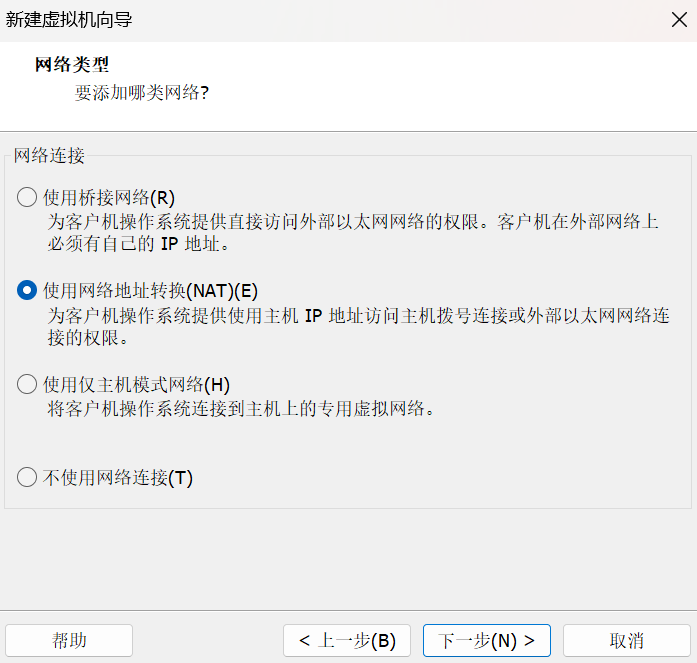
\includegraphics[width=0.95\textwidth]{picture/Screenshot 2024-10-14 113215.png}
    \caption{虚拟机创建界面}
\end{figure}
网络类型选择NAT模式,点击“下一步”。

\begin{figure}[H]
    \centering
    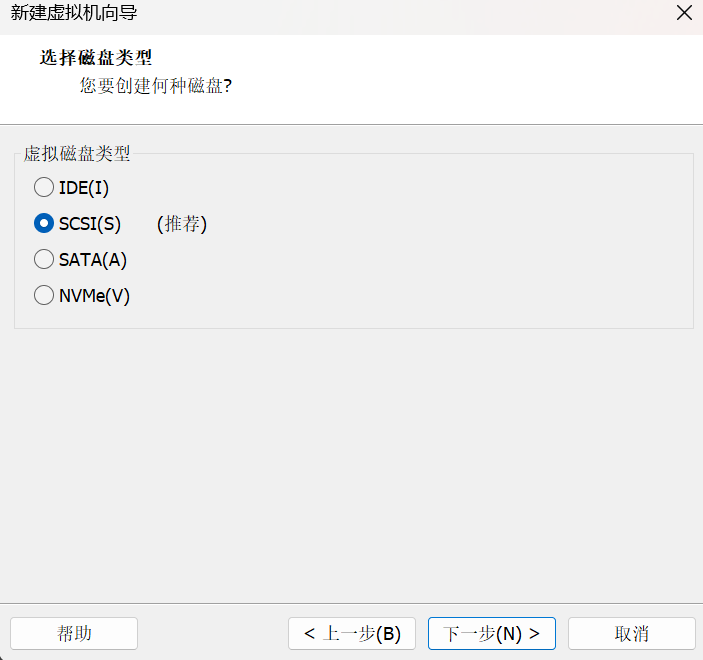
\includegraphics[width=0.95\textwidth]{picture/Screenshot 2024-10-14 113358.png}
    \caption{虚拟机创建界面}
\end{figure}
点击“下一步”。

\begin{figure}[H]
    \centering
    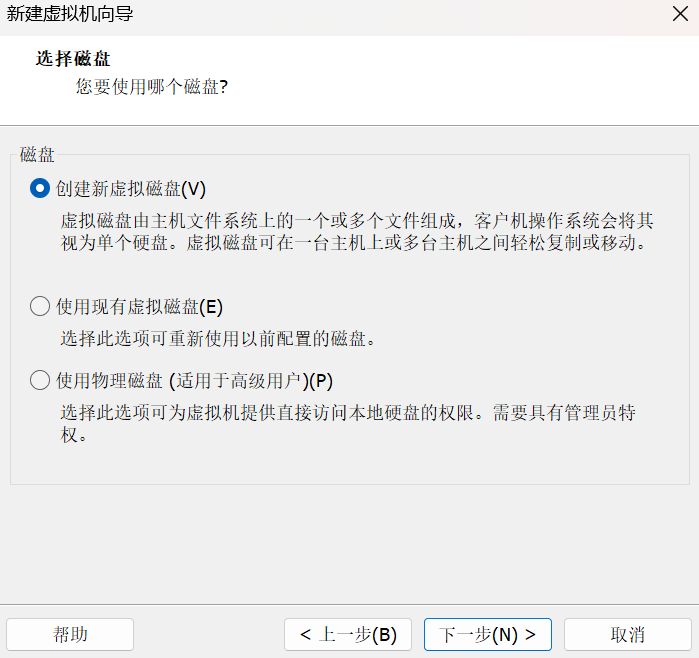
\includegraphics[width=0.95\textwidth]{picture/Screenshot 2024-10-14 113443.png}
    \caption{虚拟机创建界面}
\end{figure}
点击“下一步”。

\begin{figure}[H]
    \centering
    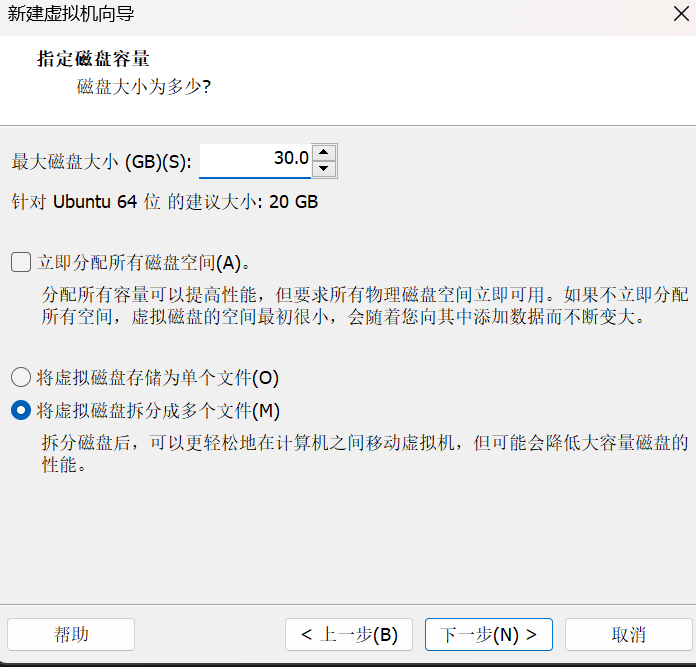
\includegraphics[width=0.95\textwidth]{picture/Screenshot 2024-10-14 113546.png}
    \caption{虚拟机创建界面}
\end{figure}
将磁盘大小修改成30GB,点击“下一步”。

\begin{figure}[H]
    \centering
    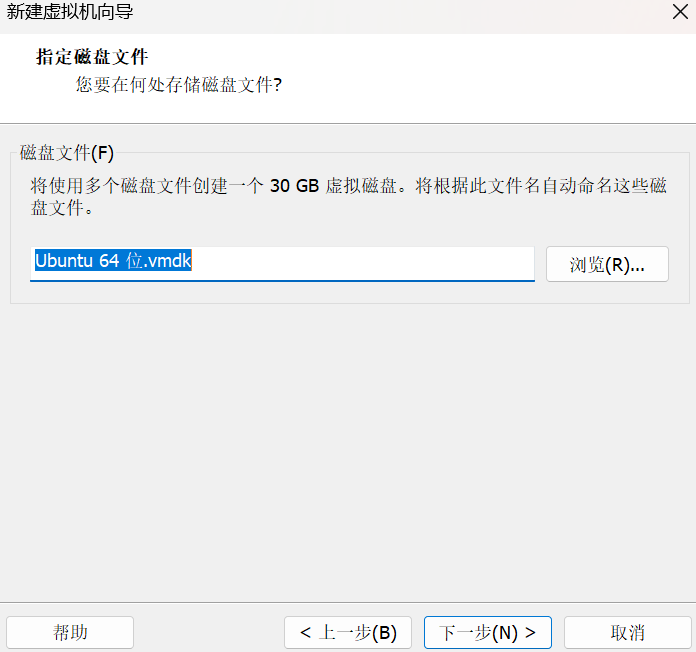
\includegraphics[width=0.95\textwidth]{picture/Screenshot 2024-10-14 113657.png}
    \caption{虚拟机创建界面}
\end{figure}
点击“下一步”。

\begin{figure}[H]
    \centering
    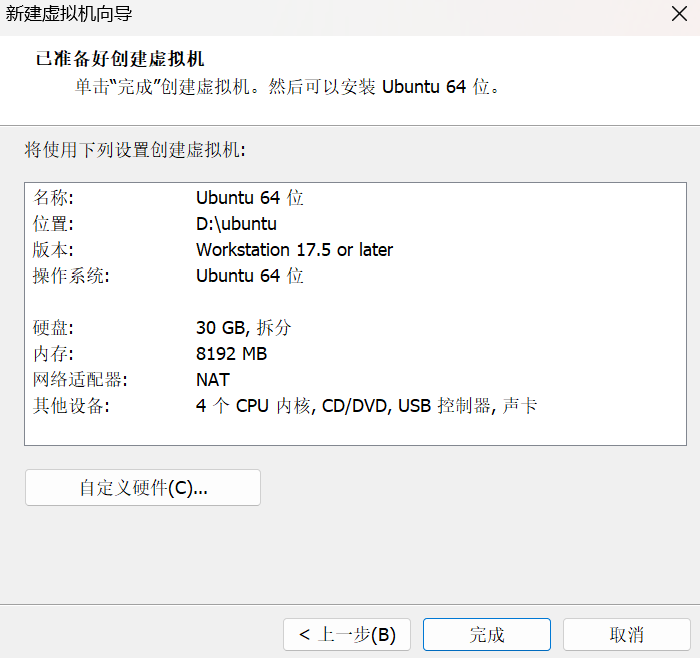
\includegraphics[width=0.95\textwidth]{picture/Screenshot 2024-10-14 113721.png}
    \caption{虚拟机创建界面}
\end{figure}
点击“完成”按钮,完成虚拟机创建。

\begin{figure}[H]
    \centering
    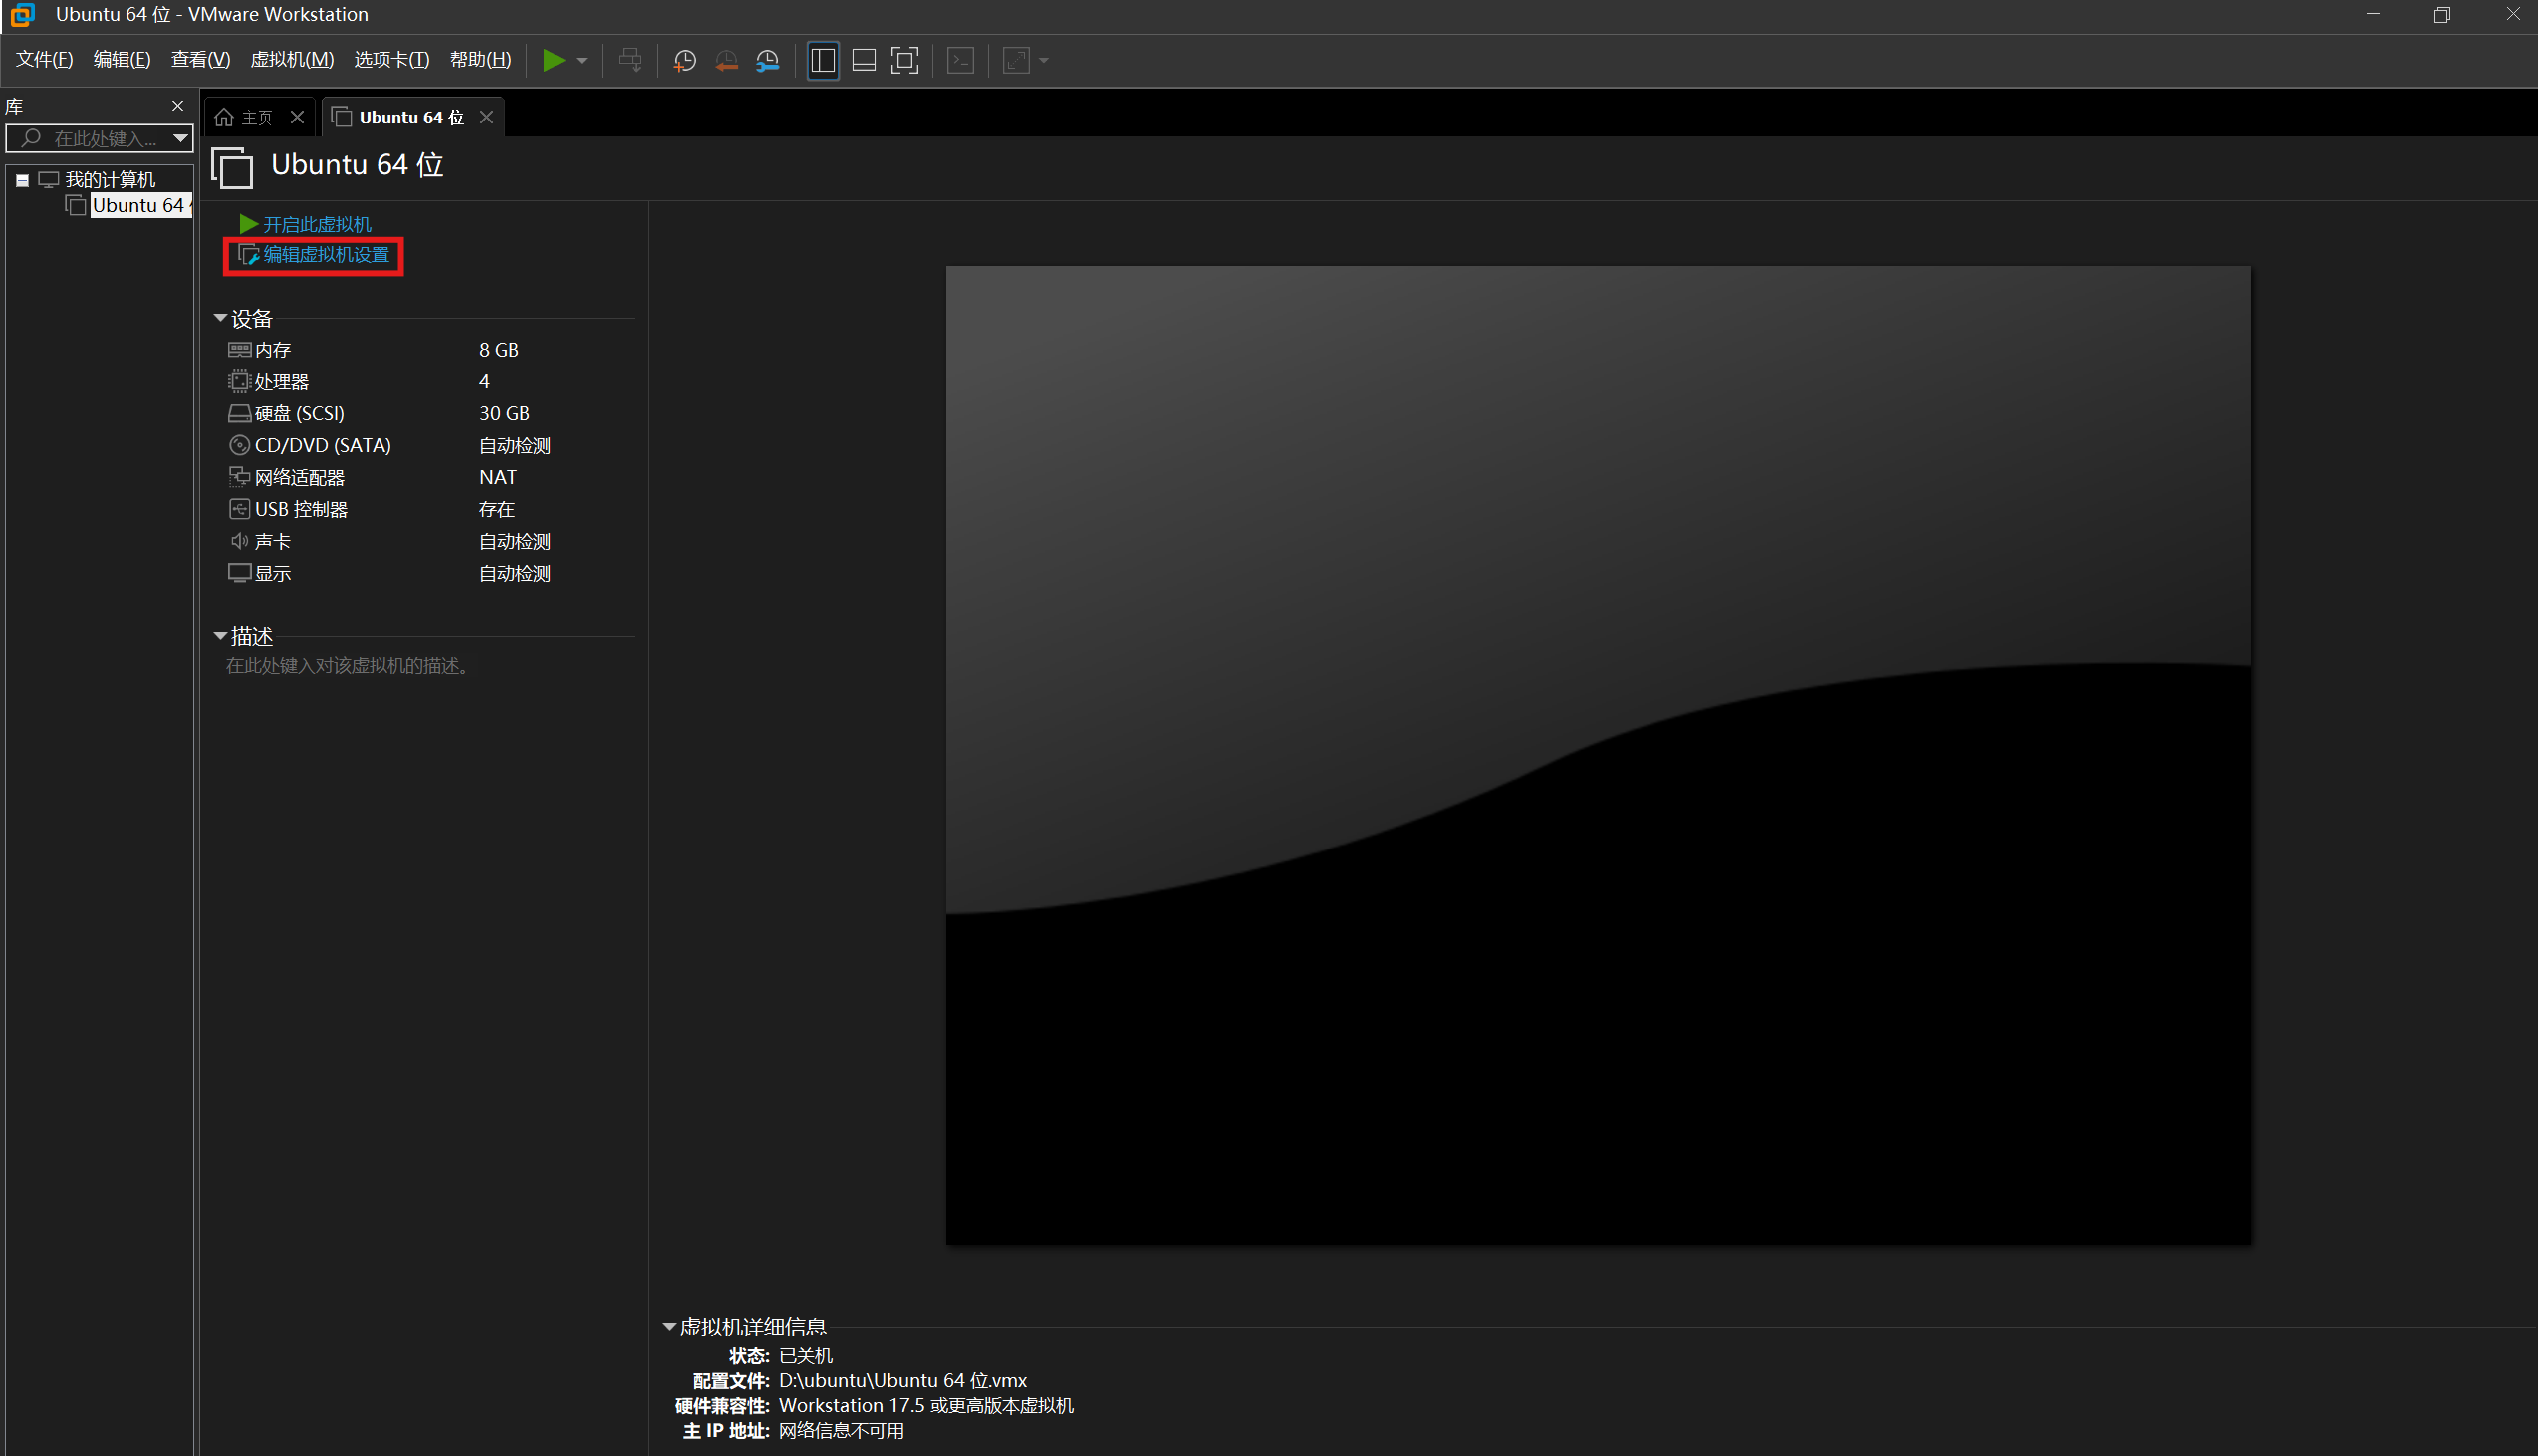
\includegraphics[width=0.95\textwidth]{picture/Screenshot 2024-10-14 113849.png}
    \caption{虚拟机界面}
\end{figure}
点击“编辑虚拟机设置”。

\begin{figure}[H]
    \centering
    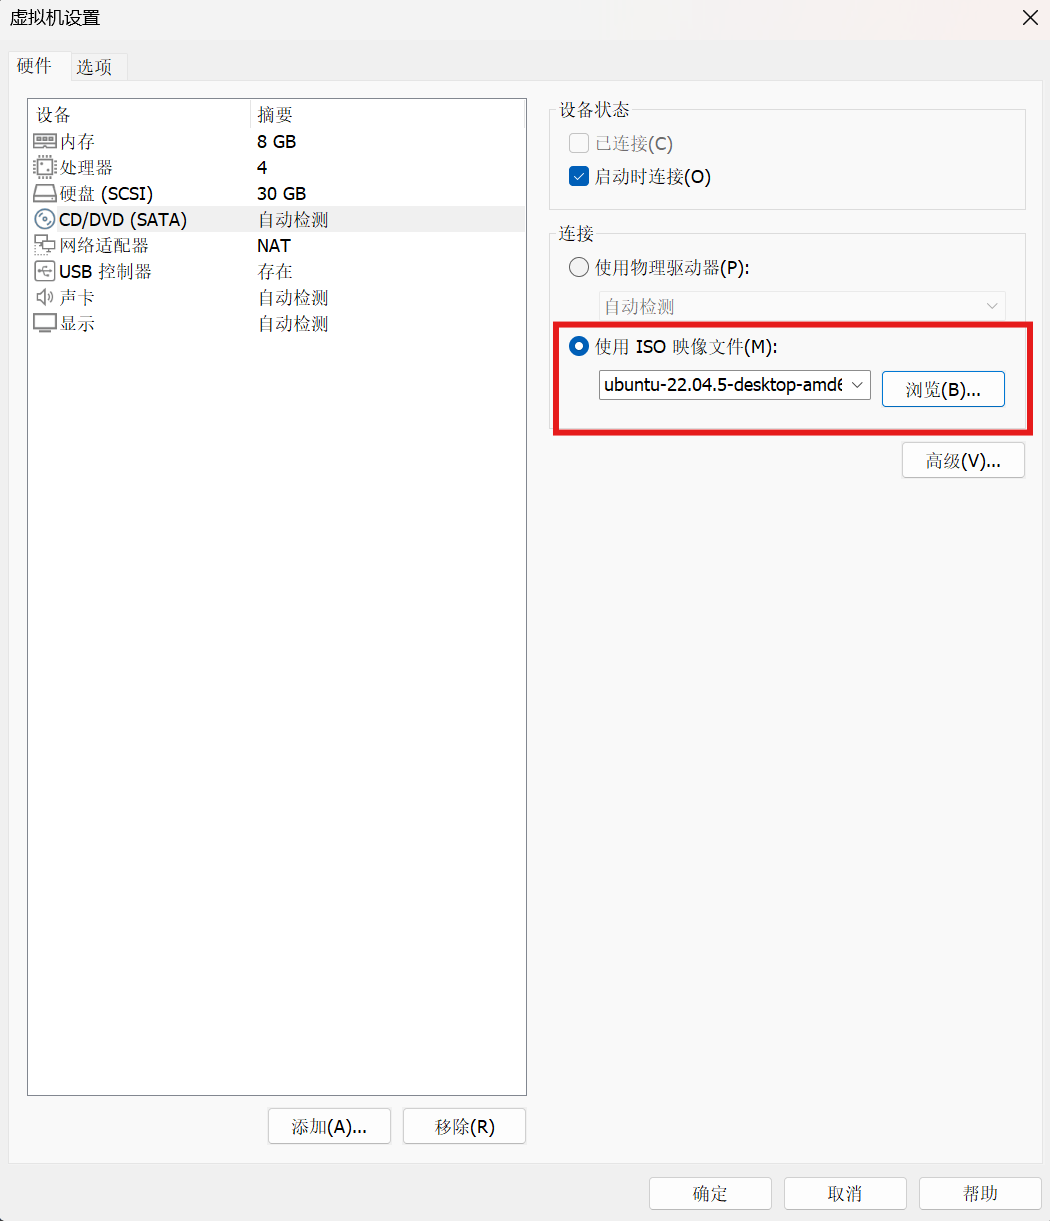
\includegraphics[width=0.95\textwidth]{picture/Screenshot 2024-10-14 114016.png}
    \caption{虚拟机设置界面}
\end{figure}
选择CD/DVD,点击“选择ISO镜像文件”,选择刚刚下载的Ubuntu 22.04 LTS amd64镜像文件,点击“打开”。

\begin{figure}[H]
    \centering
    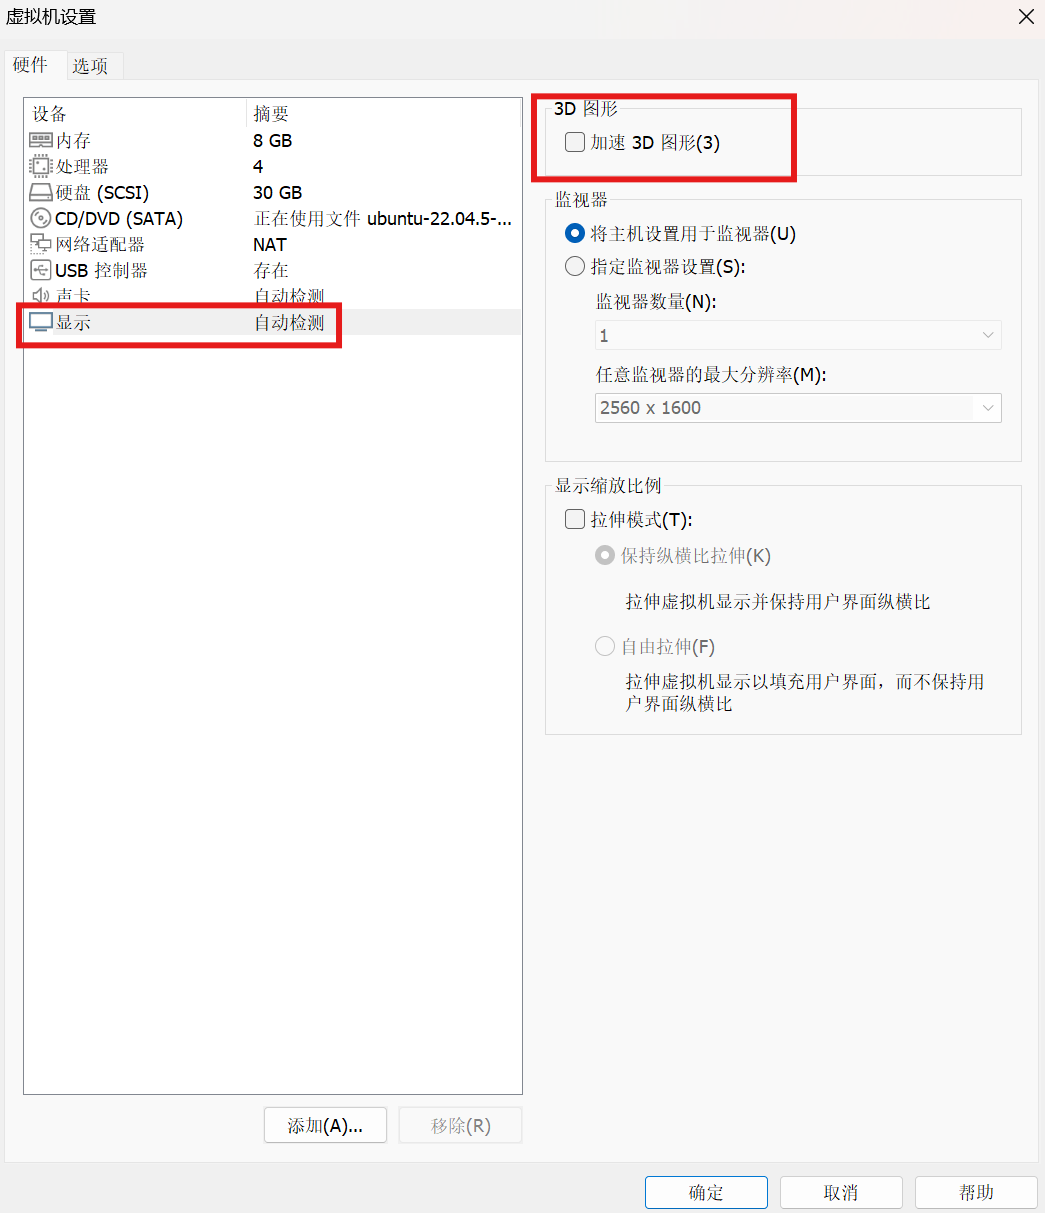
\includegraphics[width=0.95\textwidth]{picture/Screenshot 2024-10-14 114300.png}
    \caption{虚拟机设置界面}
\end{figure}
注意,如果之后出现卡顿,可以尝试在“显示”中关闭3D加速。
\\点击“确定”。
\\注意,到这一步实是把 Ubuntu 的虚拟机创建好了,并不是把 Ubuntu 系统安装了,
正式的安装需要启动虚拟机。

\begin{figure}[H]
    \centering
    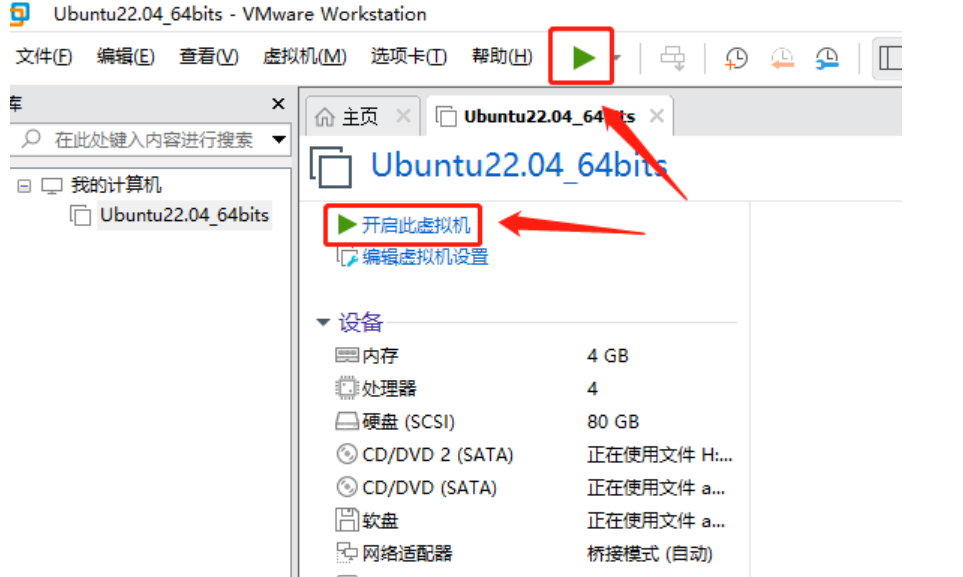
\includegraphics[width=0.95\textwidth]{picture/Screenshot 2024-10-14 160637.png}
    \caption{打开虚拟机}
\end{figure}
点击“启动”按钮,启动虚拟机。

\begin{figure}[H]
    \centering
    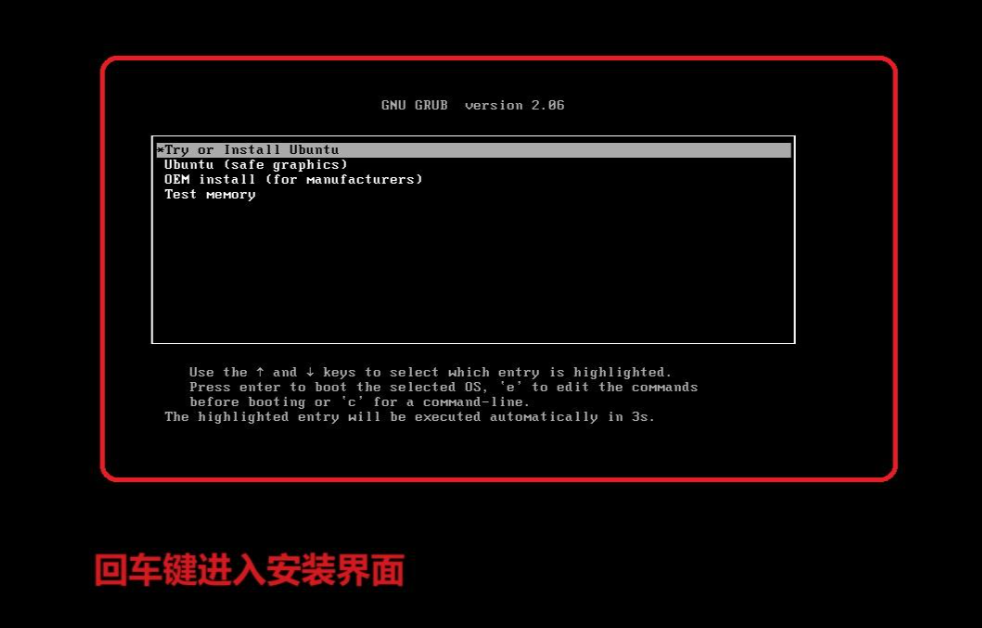
\includegraphics[width=0.95\textwidth]{picture/Screenshot 2024-10-14 173720.png}
    \caption{Ubuntu安装界面}
\end{figure}
按Enter键继续。

\begin{figure}[H]
    \centering
    
\includegraphics[width=0.95\textwidth]{picture/Screenshot 2024-10-14 174058.png}
    \caption{Ubuntu安装界面}
\end{figure}
选择语言,点击“继续”。

\begin{figure}[H]
    \centering
    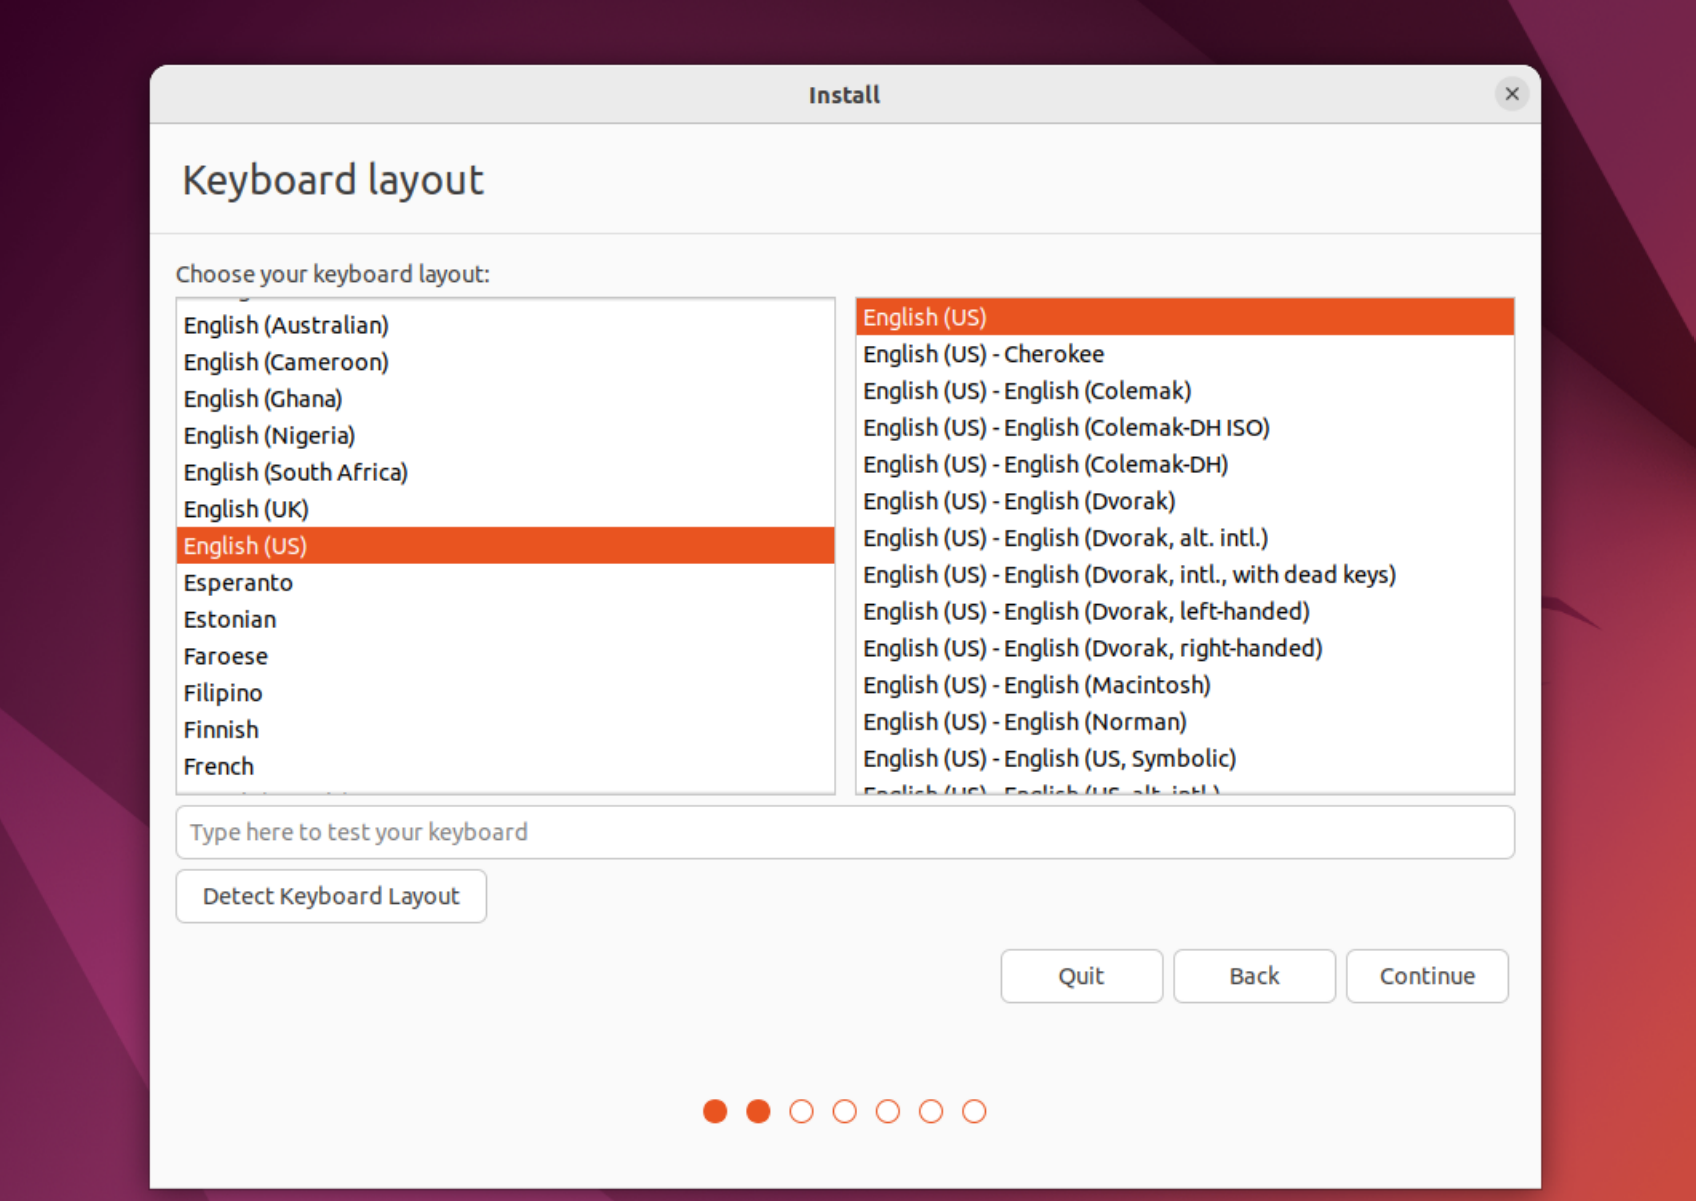
\includegraphics[width=0.95\textwidth]{picture/Screenshot 2024-10-14 174312.png}
    \caption{Ubuntu安装界面}
\end{figure}
选择键盘布局,点击“继续”。

\begin{figure}[H]
    \centering
    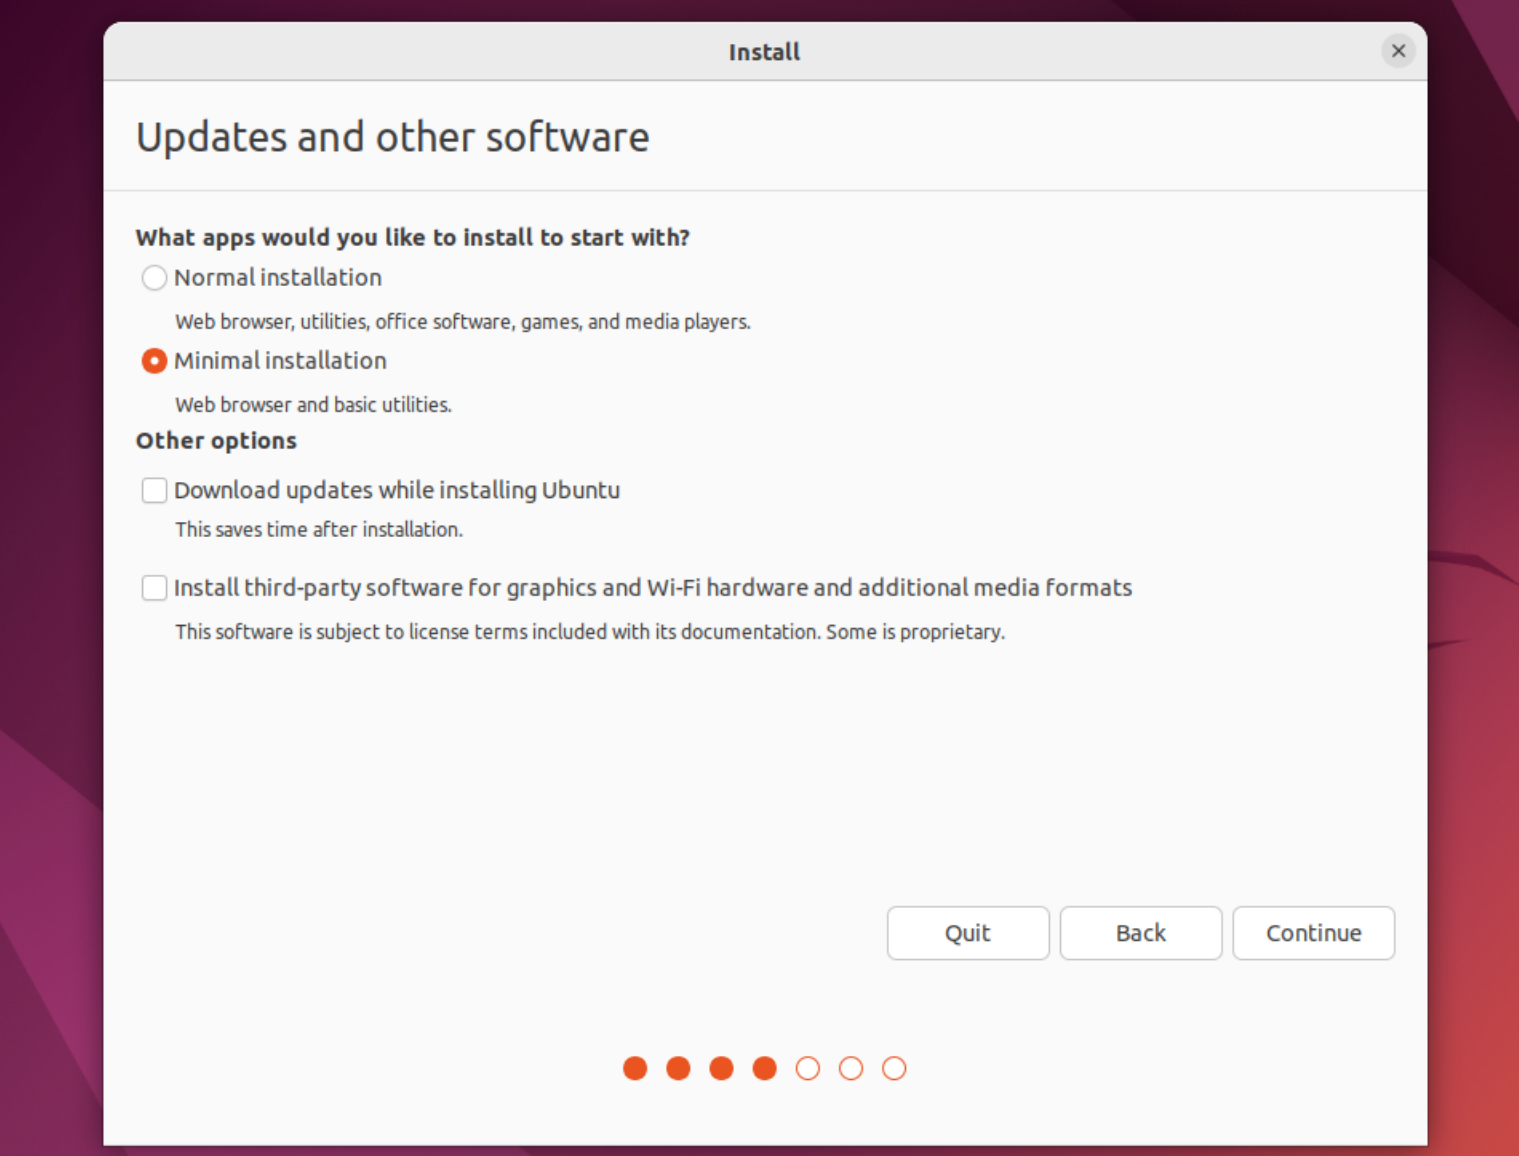
\includegraphics[width=0.95\textwidth]{picture/Screenshot 2024-10-14 175055.png}
    \caption{Ubuntu安装界面}
\end{figure}
选择最⼩安装设置,取消更新勾选。

\begin{figure}[H]
    \centering
    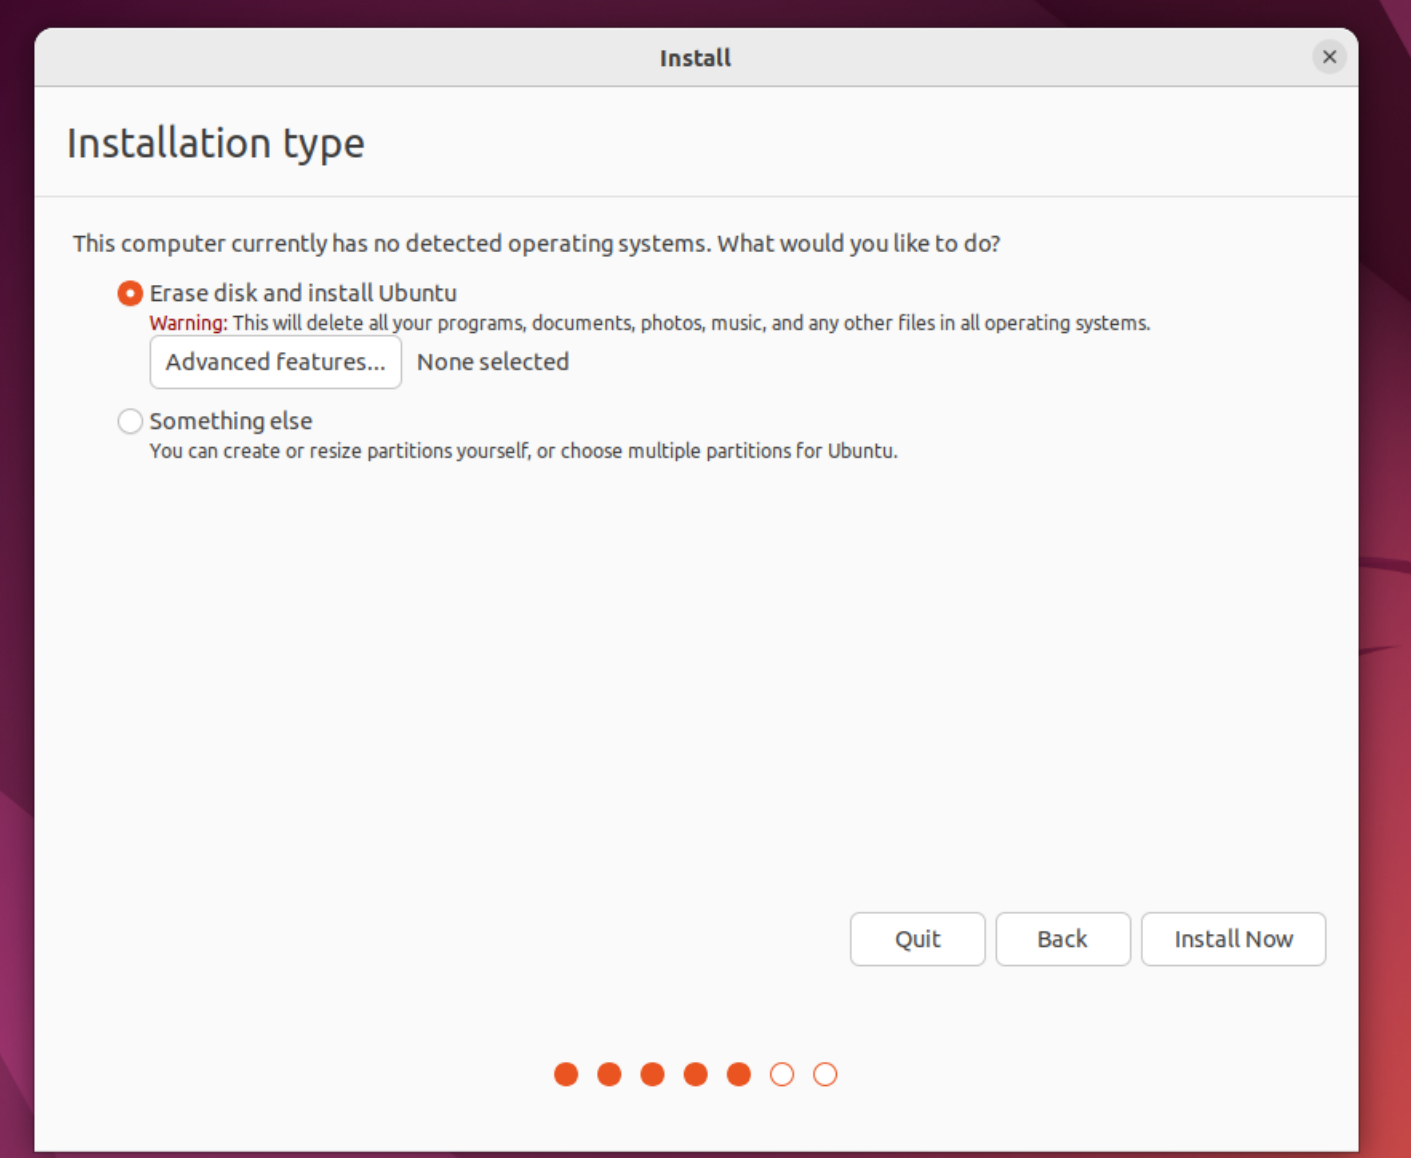
\includegraphics[width=0.95\textwidth]{picture/Screenshot 2024-10-14 174957.png}
    \caption{Ubuntu安装界面}
\end{figure}
选择安装类型,点击“继续”。

\begin{figure}[H]
    \centering
    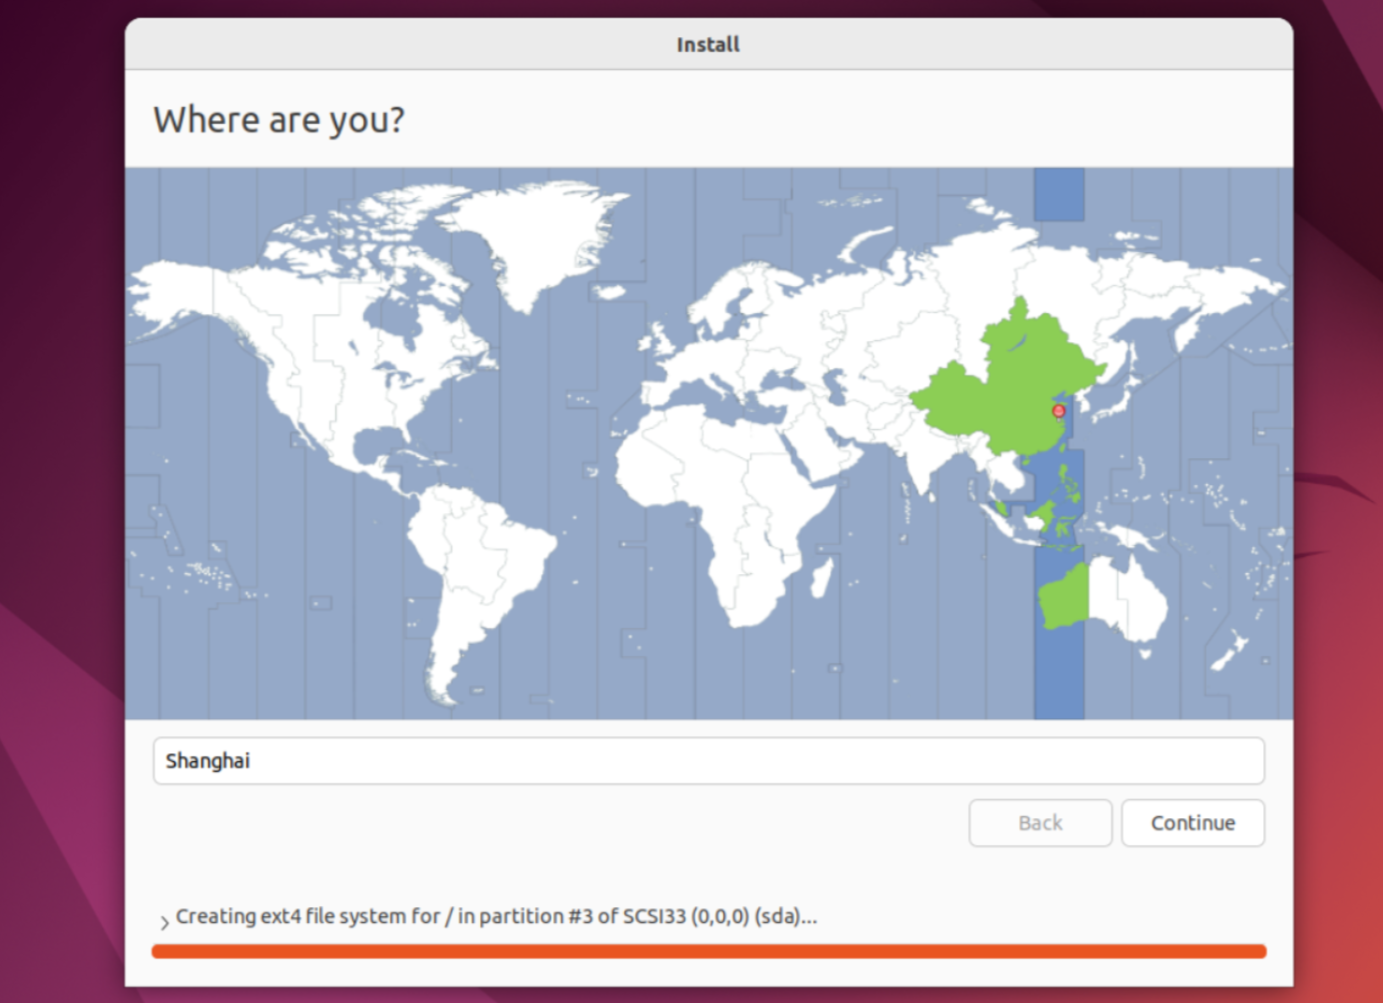
\includegraphics[width=0.95\textwidth]{picture/Screenshot 2024-10-14 192408.png}
    \caption{Ubuntu安装界面}
\end{figure}
选择时区,点击“继续”。
\\等待安装完成。

\begin{figure}[H]
    \centering
    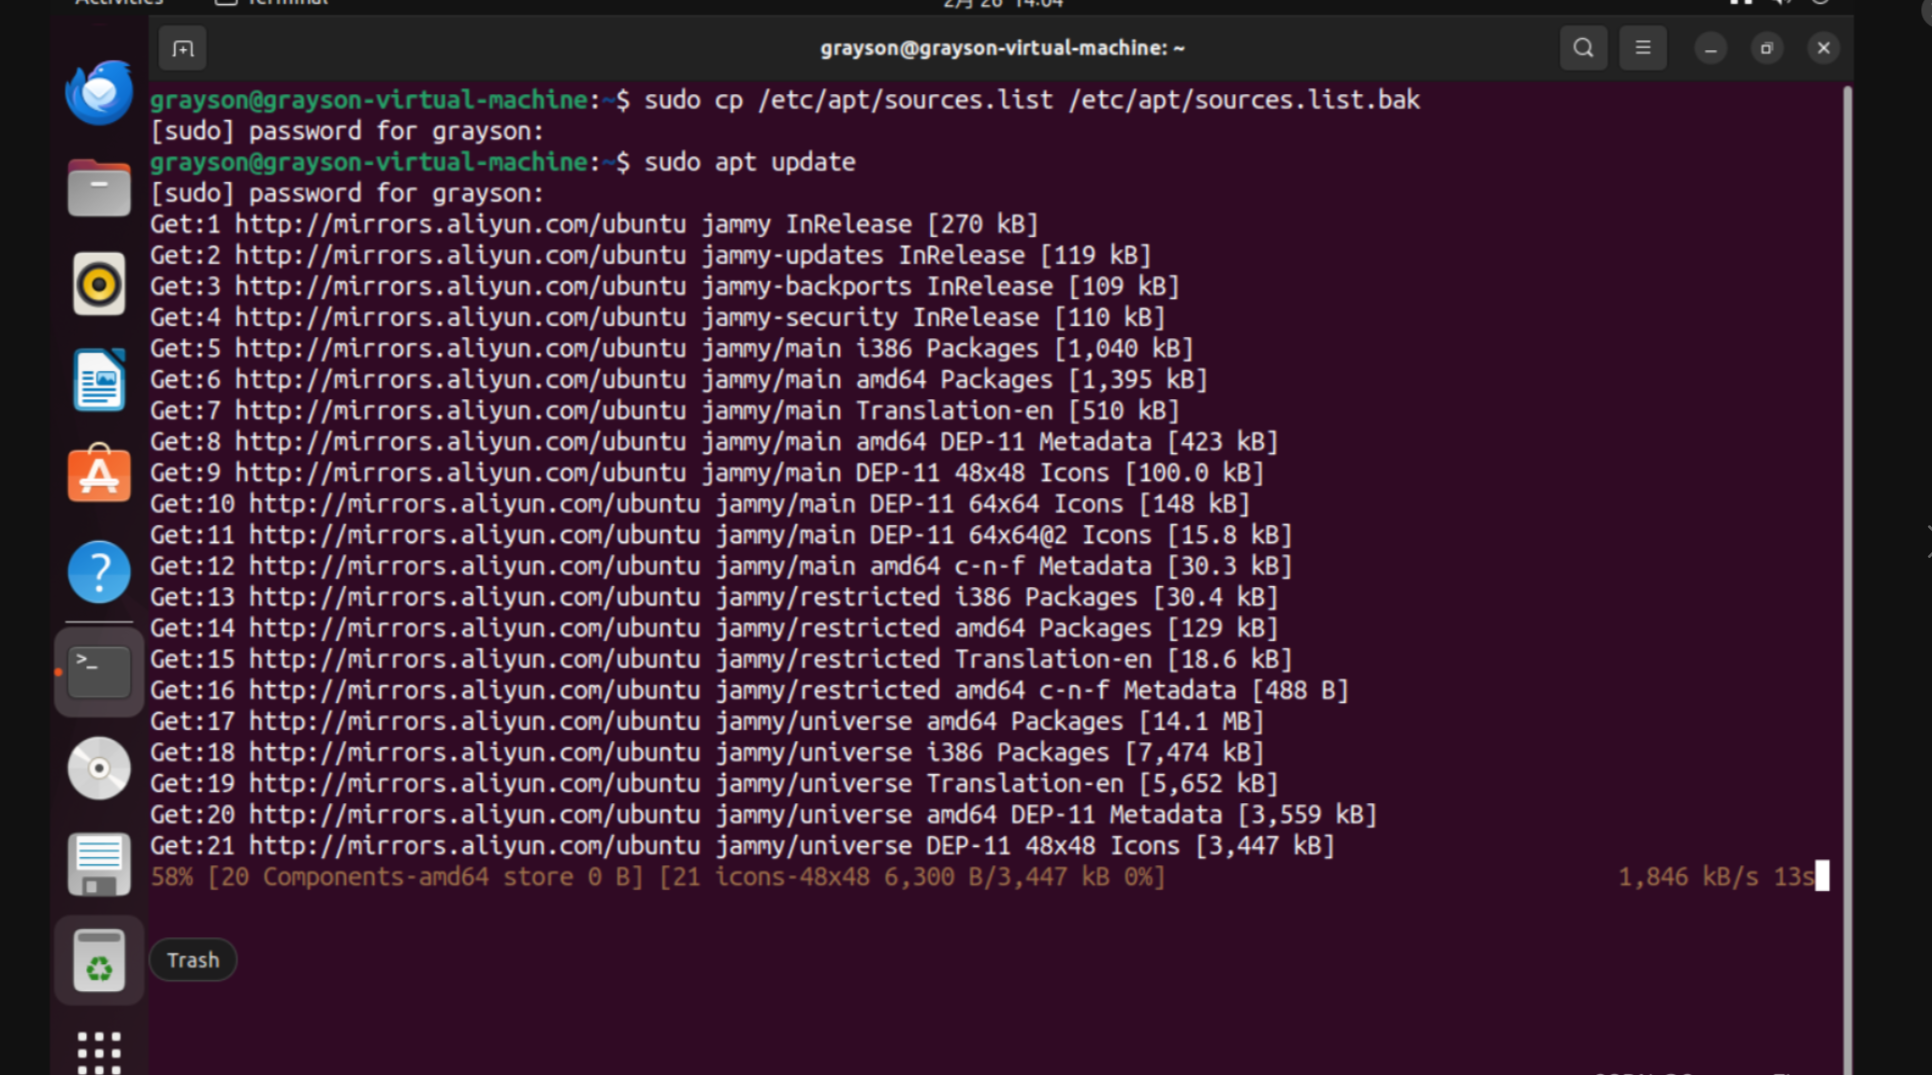
\includegraphics[width=0.95\textwidth]{picture/Screenshot 2024-10-14 193541.png}
    \caption{更新软件}
\end{figure}
更新软件,顺便验证网络连接。

\section{任务二:安装 C 语言编译器}
\subsection{任务内容}
\begin{itemize}
    \item 安装最新版本的 gcc(可通过 PPA 安装最新稳定版)。
    \item 验证编译器安装成功,并确保其正常工作。
\end{itemize}

\subsection{任务分析}
为了确保 C 语言开发环境的基础设施准备就绪,安装最新版本的 GCC 是至关重要的步
骤。通过使用 PPA(Personal Package Archive)安装最新稳定版的 GCC,可以确保
开发环境具备最新的特性和修复的 bug。首先,添加 GCC 的 PPA 源并更新软件包列表
,然后使用 `apt-get` 命令安装 GCC。安装完成后,通过 `gcc --version` 命令
检查 GCC 版本,并编写一个简单的 C 语言程序进行编译测试,以验证 GCC 是否成功安
装并正常工作。此外,还需检查 GCC 的可执行文件路径和环境变量,确保在任何目录下
都能调用 GCC。通过这些步骤,可以确保 C 语言编译器正常工作,为后续的开发工作打
下坚实的基础。

\subsection{任务实现}
\subsubsection{安装最新版本的 GCC}
\begin{figure}[H]
    \centering
    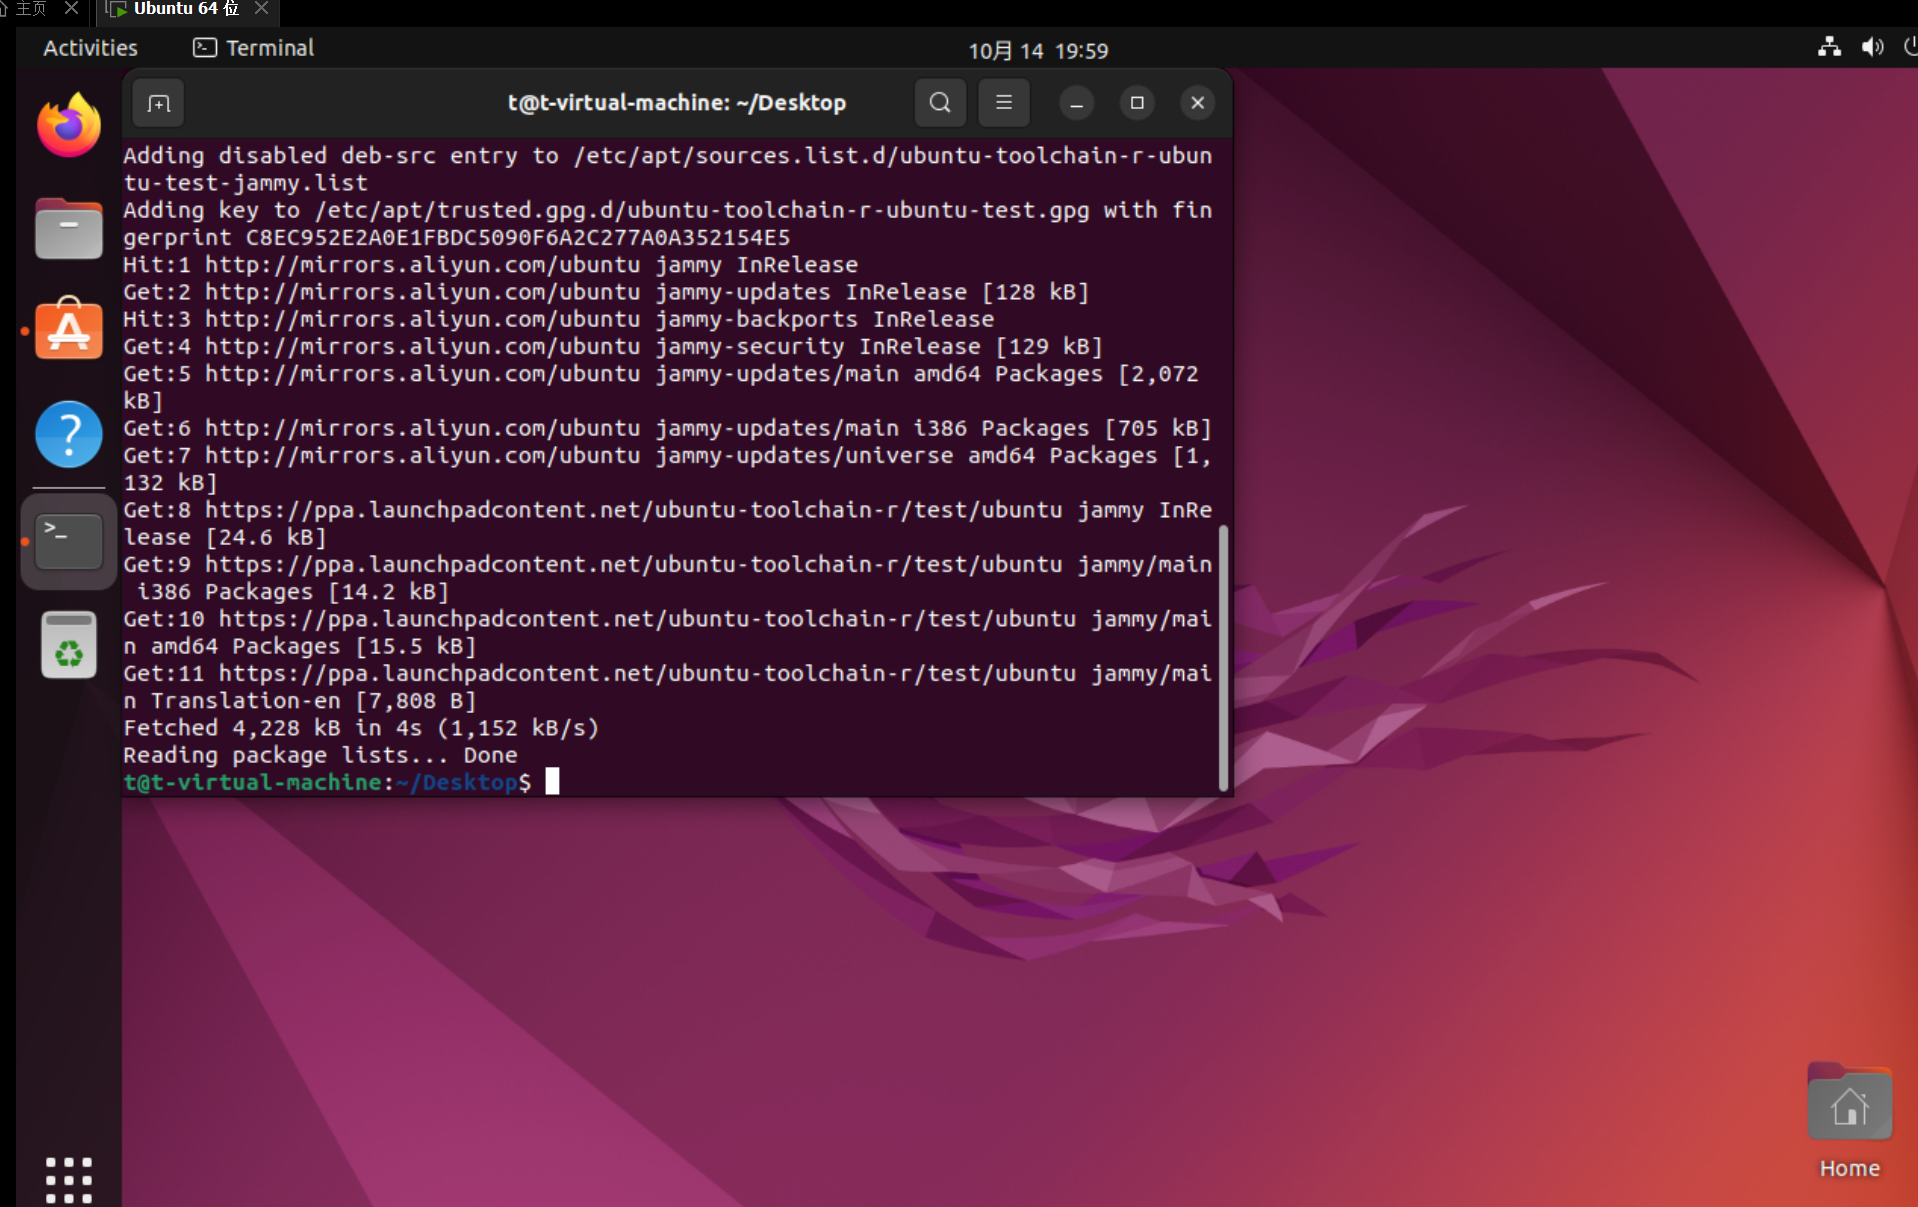
\includegraphics[width=0.95\textwidth]{picture/Screenshot 2024-10-14 200009.png}
    \caption{添加PPA源}
\end{figure}
首先,将 GCC 的 PPA 源添加到系统的软件源列表中。

\begin{figure}[H]
    \centering
    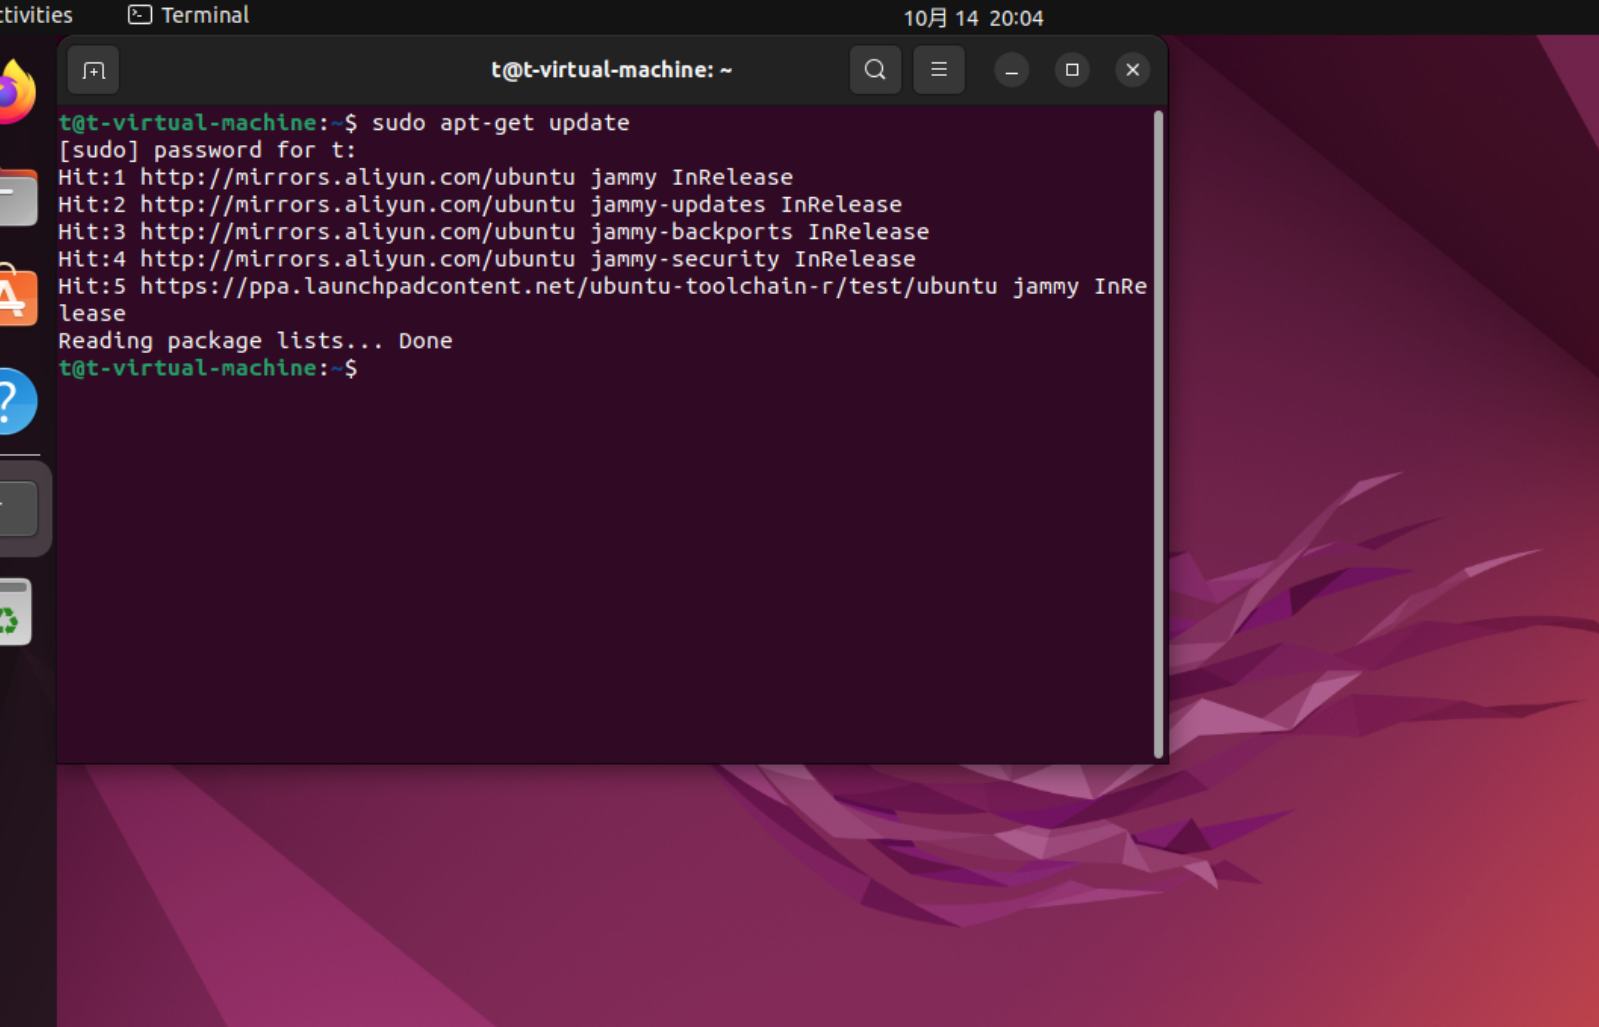
\includegraphics[width=0.95\textwidth]{picture/Screenshot 2024-10-14 200417.png}
    \caption{更新系统的软件包列表}
\end{figure}
添加 PPA 源后,更新系统的软件包列表,以确保系统能够识别新添加的软件包。

\begin{figure}[H]
    \centering
    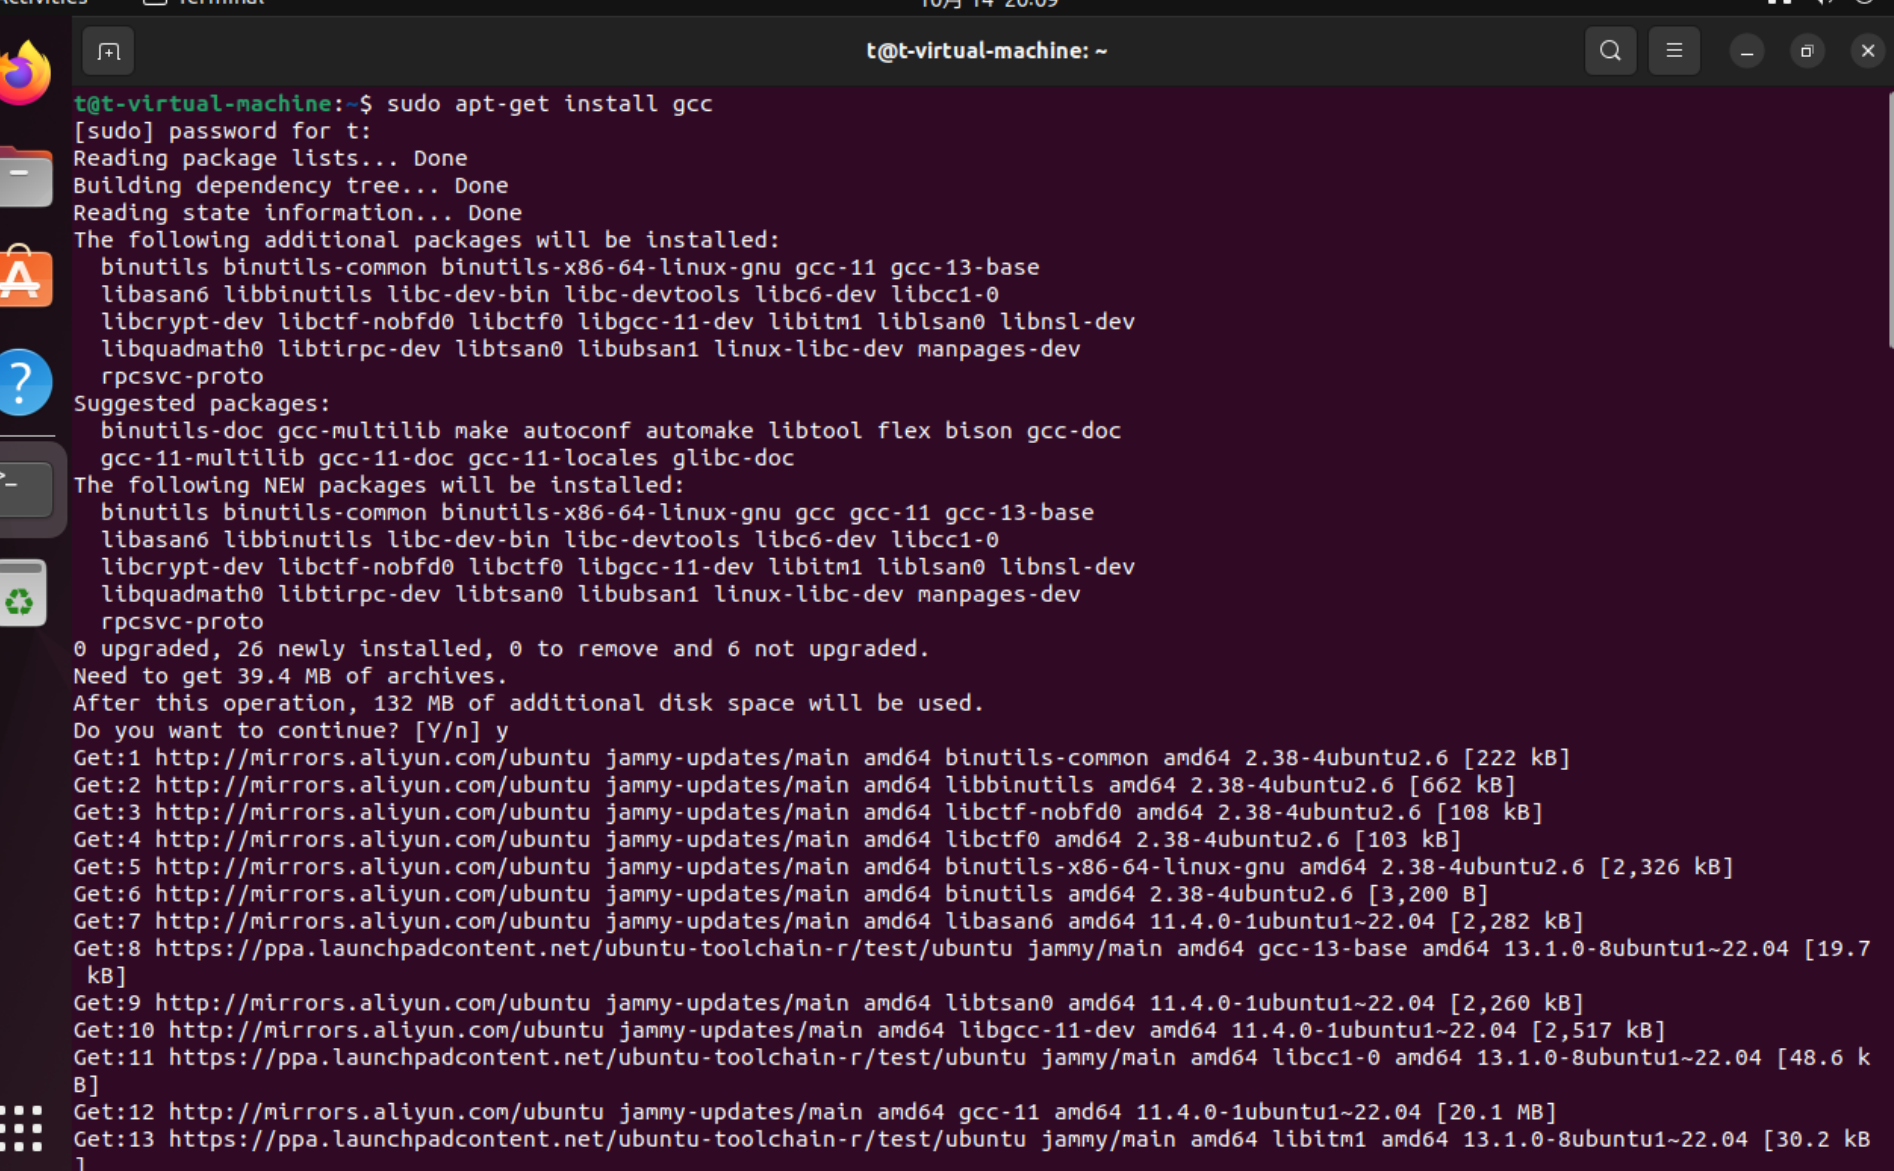
\includegraphics[width=0.95\textwidth]{picture/Screenshot 2024-10-14 200918.png}
    \caption{安装 GCC}
\end{figure}
\begin{figure}[H]
    \centering
    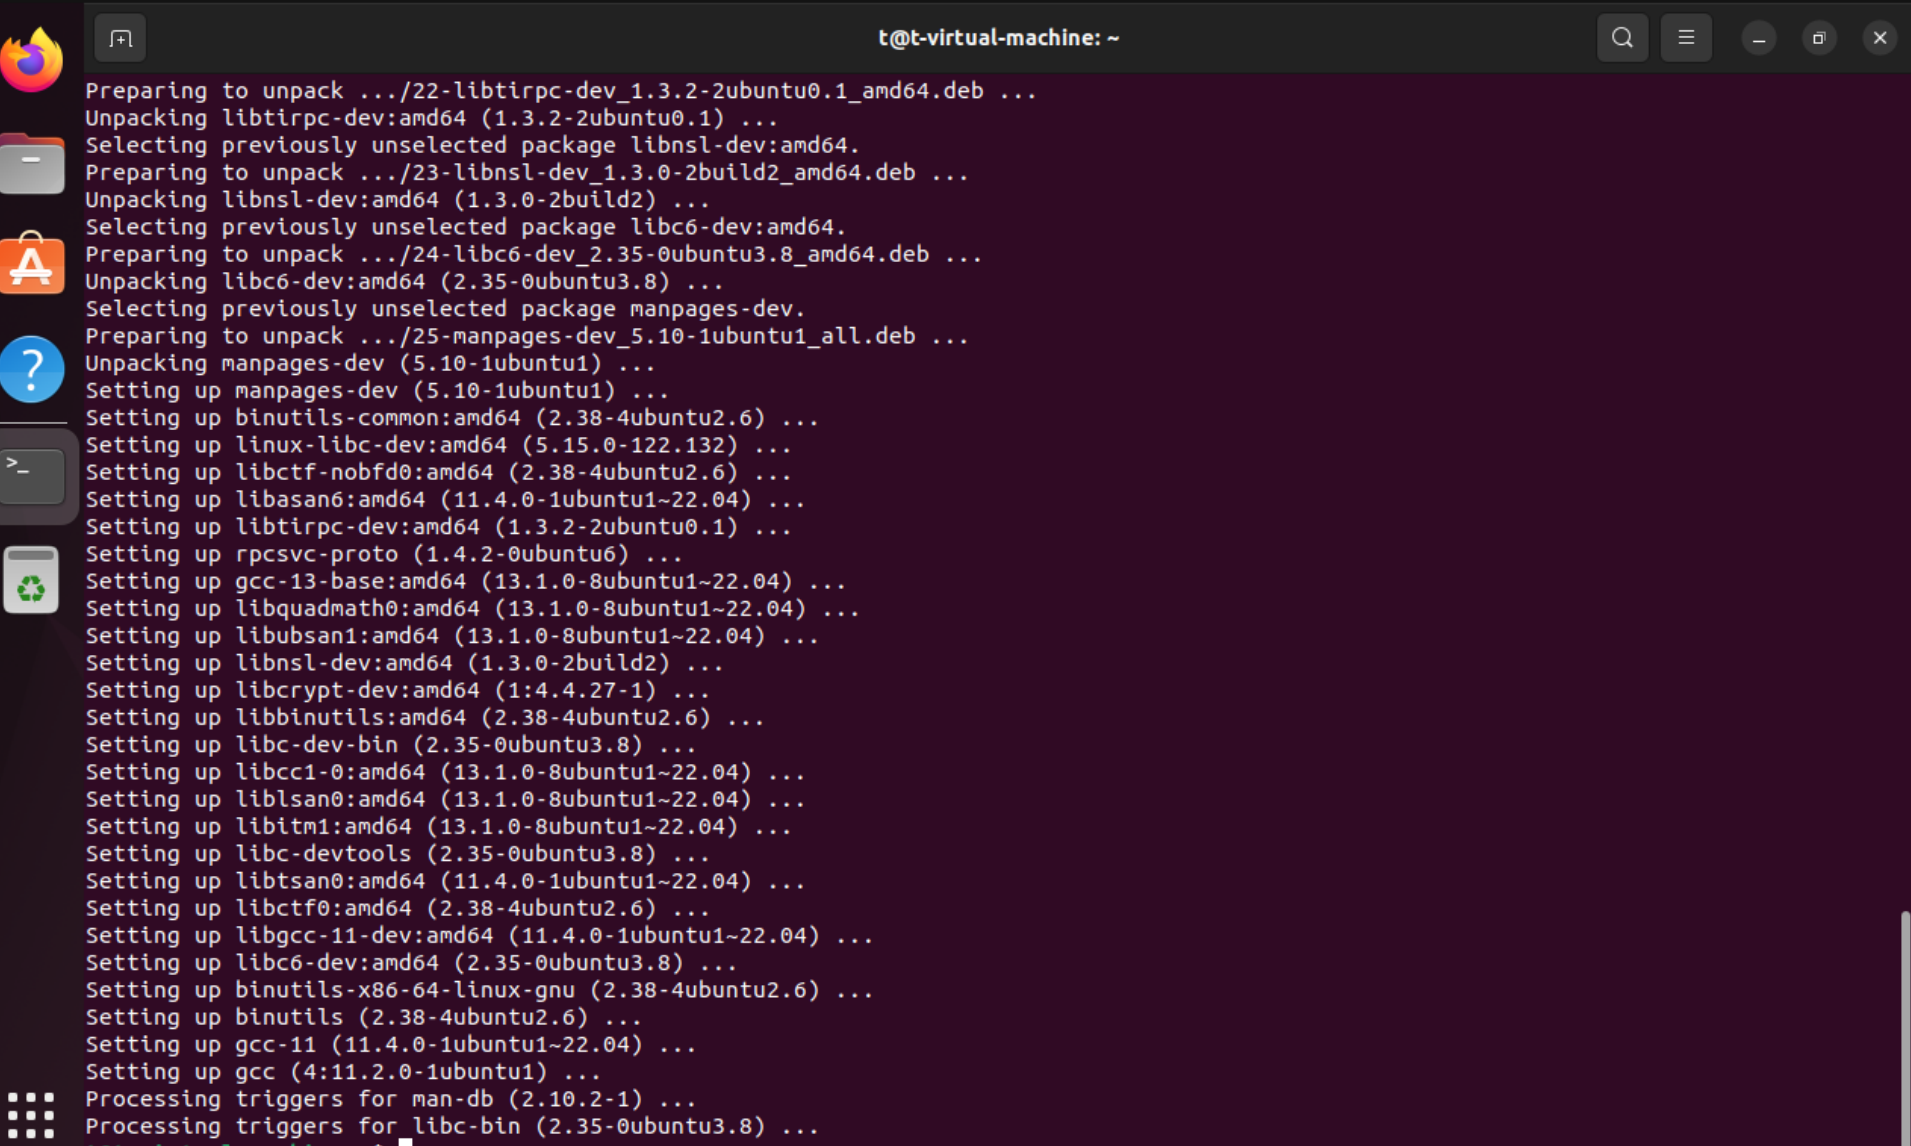
\includegraphics[width=0.95\textwidth]{picture/Screenshot 2024-10-14 200844.png}
    \caption{安装 GCC}
\end{figure}
使用 apt-get 或 apt 命令来安装 GCC。安装过程中,系统会自动解决依赖关系并下载所需的软件包。

\subsubsection{验证编译器安装成功}
\begin{figure}[H]
    \centering
    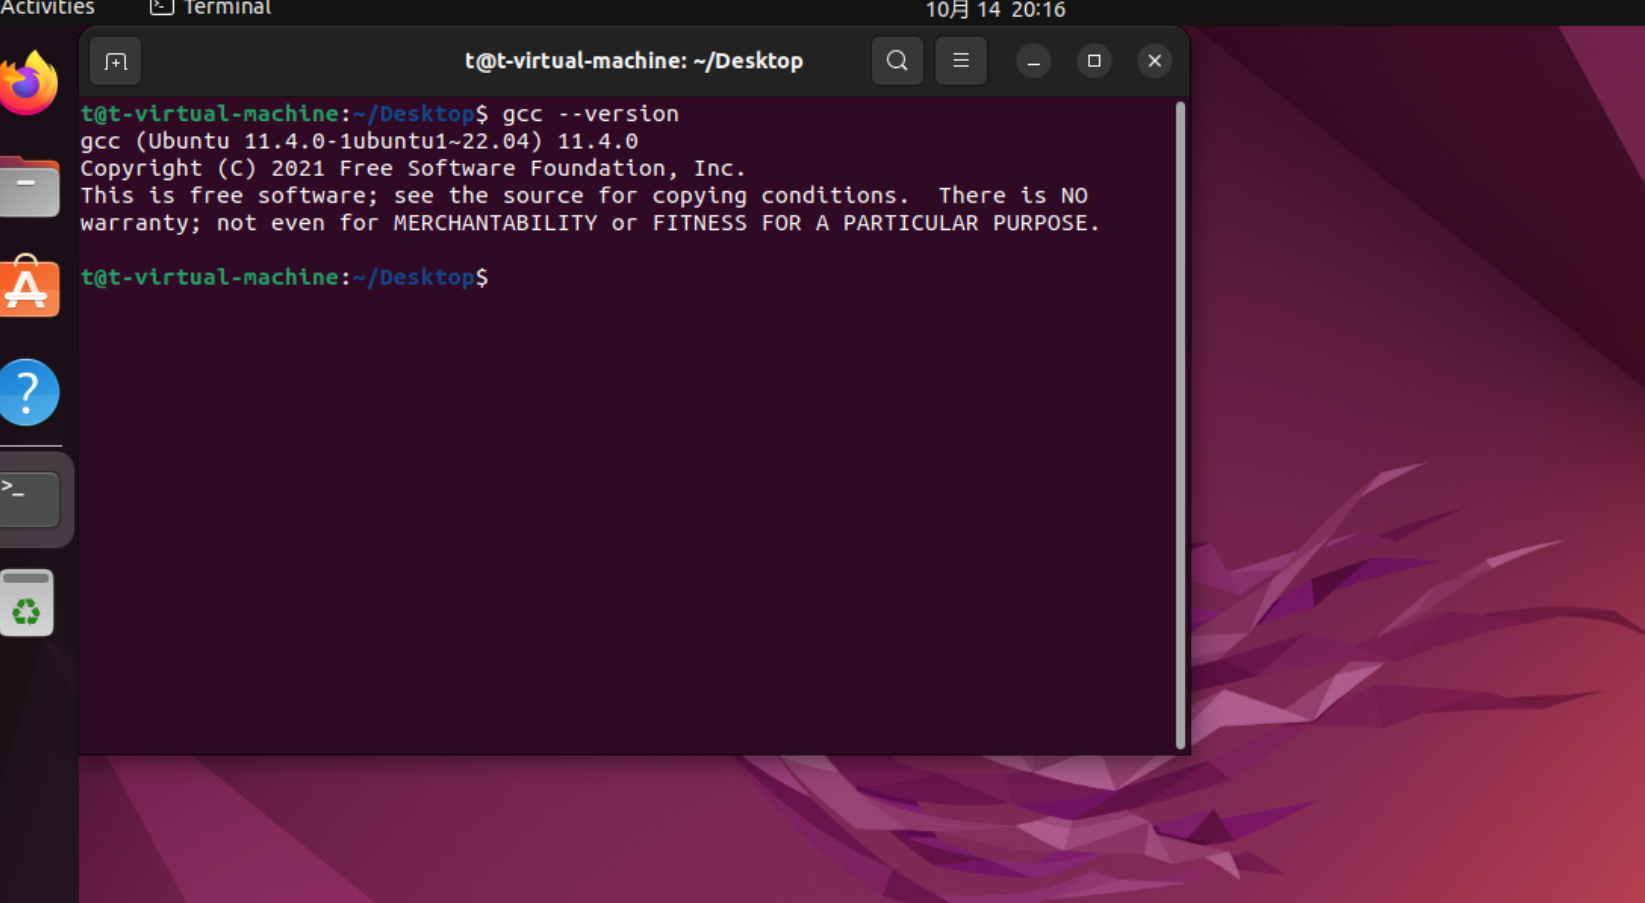
\includegraphics[width=0.95\textwidth]{picture/Screenshot 2024-10-14 201650.png}
    \caption{检查 GCC 版本}
\end{figure}
使用 gcc --version 命令来查看已安装的 GCC 版本。

\begin{figure}[H]
    \centering
    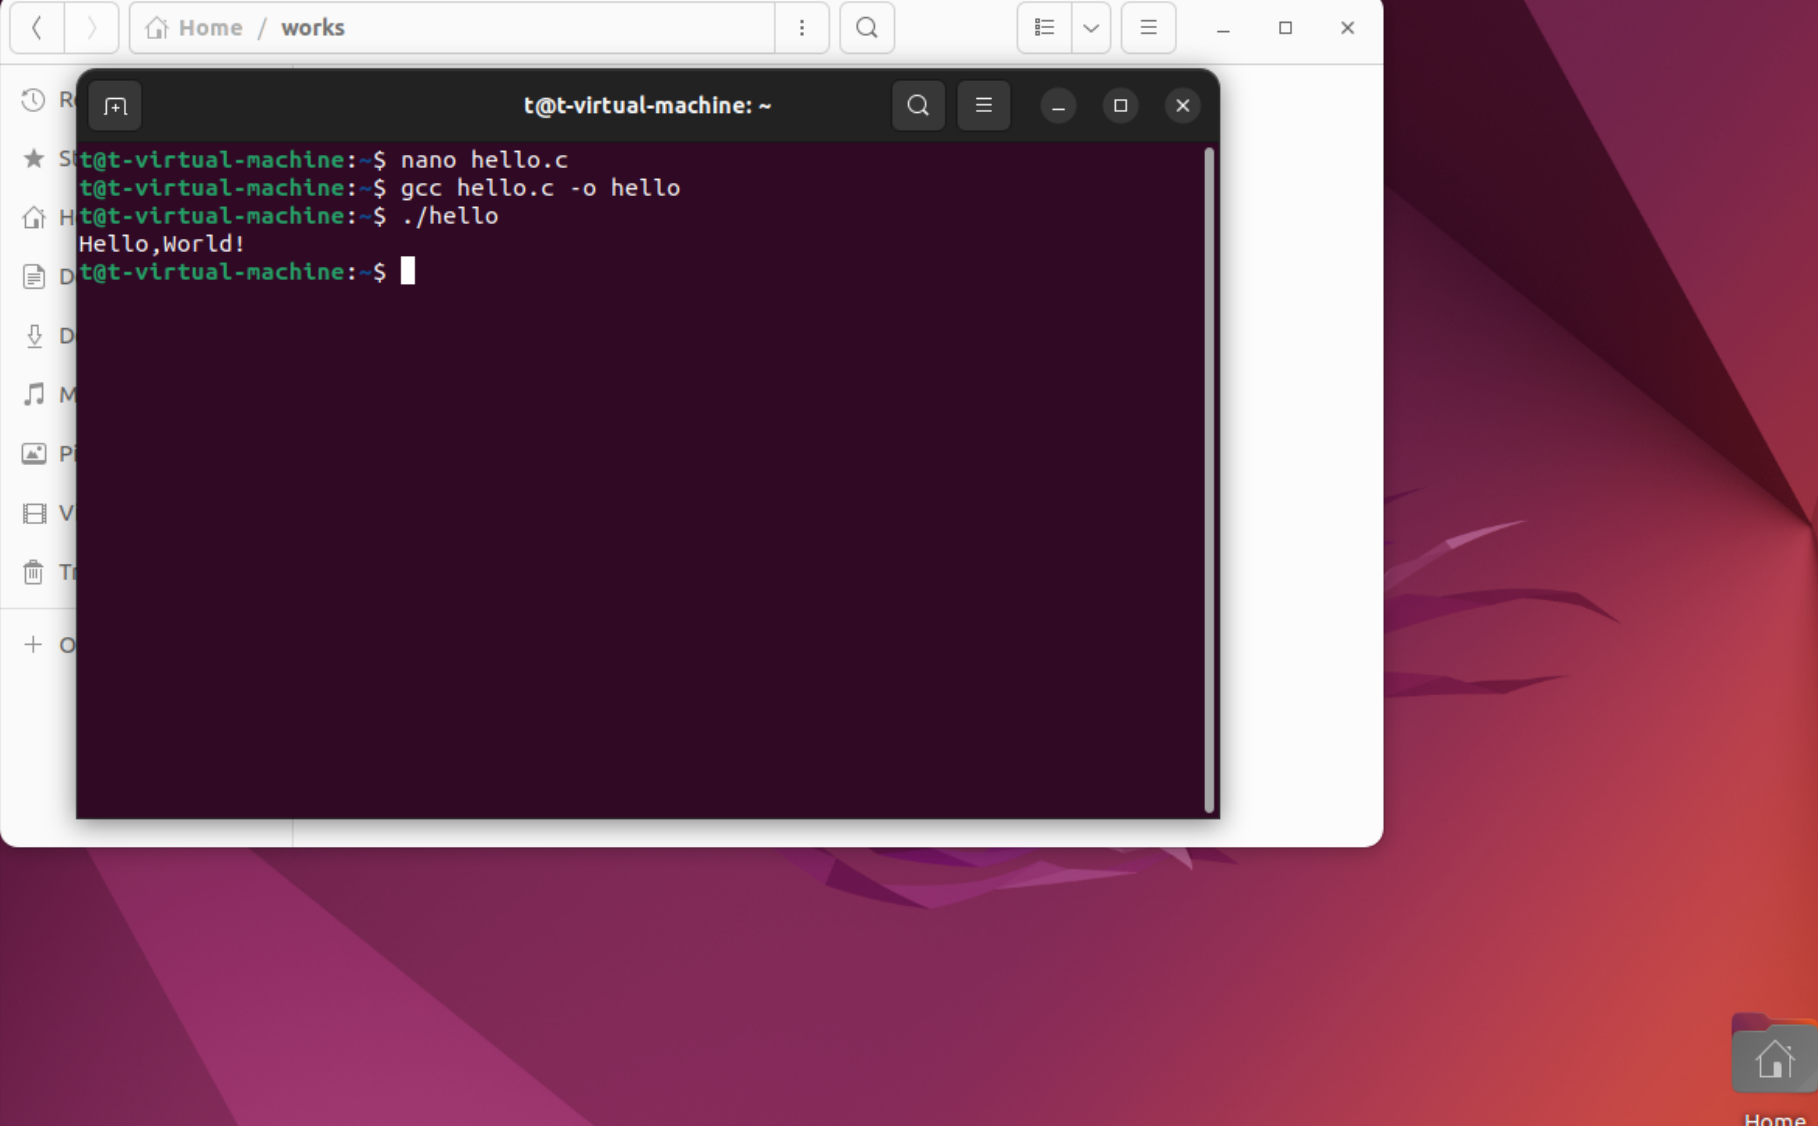
\includegraphics[width=0.95\textwidth]{picture/Screenshot 2024-10-14 203120.png}
    \caption{编译测试程序}
\end{figure}
编写一个简单的 C 语言程序(例如 hello.c),并使用 gcc 命令进行编译。如果编译成功并生成可执行文件,说明 GCC 能够正常工作。

\section{任务三:实现排序算法}
\subsection{任务内容}
\begin{itemize}
    \item 使用 C 语言手动实现以下排序算法:冒泡排序、基础堆排序以及斐波
    那契堆排序,不调用任何库函数。
    \item 运行测试代码,确认各排序算法的正确性。
\end{itemize}

\subsection{任务分析}
在本任务中,目标是在C语言环境中手动实现三种排序算法:冒泡排序、基础堆排序和斐
波那契堆排序,且不依赖任何库函数。这要求开发者不仅要理解每种算法的原理,还要能
够将其逻辑转化为C语言代码。关键步骤包括:首先,编写冒泡排序算法,利用简单的迭
代比较和交换实现排序;其次,实现基础堆排序,这涉及到构建最大堆和通过堆调整实现
排序;最后,实现更复杂的斐波那契堆排序,需要构建斐波那契堆并实现堆的合并和调整
操作。潜在挑战在于堆排序算法的逻辑复杂性,尤其是斐波那契堆的实现,这要求对数据
结构有深入的理解。建议的解决方案是分步骤实现,首先确保冒泡排序的正确性,然后逐
步过渡到更复杂的堆排序算法,并在每个阶段进行充分的测试,以验证算法的正确性和效
率。通过这种方法,可以确保最终实现的排序算法既正确又高效。

\subsection{任务实现}
\subsubsection{冒泡排序}
冒泡排序是一种简单直观的排序算法。它重复地走访过要排序的数列,
一次比较两个元素,如果他们的顺序错误就把他们交换过来。

\begin{lstlisting}
    #include <stdio.h>
    #include <stdlib.h>
    
    // 使用冒泡排序算法对数组进行排序
    void bubbleSort(float arr[], int n) {
        int i, j;
        for (i = 0; i < n-1; i++) {
            for (j = 0; j < n-i-1; j++) {
                if (arr[j] > arr[j+1]) {
                    // 交换 arr[j] 和 arr[j+1]
                    float temp = arr[j];
                    arr[j] = arr[j+1];
                    arr[j+1] = temp;
                }
            }
        }
    }
    
    // 打印数组中的元素
    void printArray(float arr[], int size) {
        int i;
        for (i = 0; i < size; i++)
            printf("%f ", arr[i]);
        printf("\n");
    }
    
    // 主函数,程序的入口
    int main() {
        FILE *file;
        char filename[] = "random_data_100000.txt"; // 文件名
        float *arr; // 使用动态内存分配
        int n = 0; // 数组中元素的数量
    
        // 打开文件
        file = fopen(filename, "r");
        if (file == NULL) {
            printf("无法打开文件 %s\n", filename);
            return 1;
        }
    
        // 动态分配内存
        arr = (float *)malloc(100000 * sizeof(float));
        if (arr == NULL) {
            printf("内存分配失败\n");
            fclose(file);
            return 1;
        }
    
        // 读取文件中的浮点数
        while (fscanf(file, "%f", &arr[n]) != EOF) {
            n++;
        }
    
        // 关闭文件
        fclose(file);
    
        // 对数组进行排序
        bubbleSort(arr, n);
    
        // 打印排序后的数组
        printf("Sorted array: \n");
        printArray(arr, n);
    
        // 释放内存
        free(arr);
    
        return 0;
    }
\end{lstlisting}

测试代码运行效果
\begin{figure}[H]
    \centering
    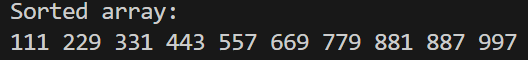
\includegraphics[width=0.95\textwidth]{picture/Screenshot 2024-10-20 155754.png}
    \caption{冒泡排序效果}
\end{figure}

\subsubsection{基础堆排序}
基础堆排序是堆排序的一种实现方式。它利用了堆数据结构,首先将待排序的数
据构建成一个堆,然后从堆顶开始,将最大的元素(堆顶元素)与堆的最后一个
元素交换,然后将剩余的元素重新构造成一个堆,重复这个过程,直到所有元素都
排序完成。

\begin{lstlisting}
    #include <stdio.h>
    #include <stdlib.h>
    
    void swap(float* a, float* b) {
        float temp = *a;
        *a = *b;
        *b = temp;
    }
    
    void heapify(float arr[], int n, int i) {
        int largest = i;
        int left = 2 * i + 1;
        int right = 2 * i + 2;
    
        if (left < n && arr[left] > arr[largest])
            largest = left;
    
        if (right < n && arr[right] > arr[largest])
            largest = right;
    
        if (largest != i) {
            swap(&arr[i], &arr[largest]);
            heapify(arr, n, largest);
        }
    }
    
    void heapSort(float arr[], int n) {
        for (int i = n / 2 - 1; i >= 0; i--)
            heapify(arr, n, i);
    
        for (int i = n - 1; i > 0; i--) {
            swap(&arr[0], &arr[i]);
            heapify(arr, i, 0);
        }
    }
    
    void printArray(float arr[], int size) {
        for (int i = 0; i < size; i++)
            printf("%.2f ", arr[i]);
        printf("\n");
    }
    
    int main() {
        FILE *file;
        char filename[] = "random_data_100000.txt";
        float *arr;
        int n = 0;
        int capacity = 100000; // 初始容量设置为 100,000
    
        // 动态分配内存
        arr = (float *)malloc(capacity * sizeof(float));
        if (arr == NULL) {
            printf("内存分配失败\n");
            return 1;
        }
    
        // 打开文件
        file = fopen(filename, "r");
        if (file == NULL) {
            printf("无法打开文件 %s\n", filename);
            free(arr);
            return 1;
        }
    
        // 读取文件中的浮点数
        while (fscanf(file, "%f", &arr[n]) != EOF) {
            n++;
            if (n >= capacity) {
                capacity *= 2;
                arr = (float *)realloc(arr, capacity * sizeof(float));
                if (arr == NULL) {
                    printf("内存重新分配失败\n");
                    fclose(file);
                    return 1;
                }
            }
        }
    
        // 关闭文件
        fclose(file);
    
        // 对数组进行排序
        heapSort(arr, n);
    
        // 打印排序后的数组
        printf("Sorted array: \n");
        printArray(arr, n);
    
        // 释放内存
        free(arr);
    
        return 0;
    }
\end{lstlisting}

测试代码运行效果
\begin{figure}[H]
    \centering
    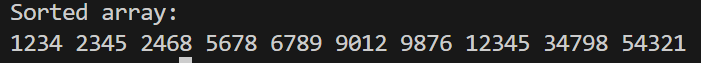
\includegraphics[width=0.95\textwidth]{picture/Screenshot 2024-10-20 162055.png}
    \caption{基础堆排序效果}
\end{figure}

\subsubsection{斐波那契堆排序}
斐波那契堆排序是堆排序的一种实现方式。它利用了斐波那契堆数据结构,首先将待
排序的数据构建成一个斐波那契堆,然后从堆顶开始,将最大的元素(堆顶元素)与
堆的最后一个元素交换,然后将剩余的元素重新构造成一个斐波那契堆,重复这个
过程,直到所有元素都排序完成。

\begin{lstlisting}
    #include <stdio.h>
    #include <stdlib.h>
    #include <math.h>
    #include <float.h>
    
    typedef int Type;
    
    typedef struct _FibonacciNode {
        Type   key;                        // 关键字(键值)
        int degree;                        // 度数
        struct _FibonacciNode *left;       // 左兄弟
        struct _FibonacciNode *right;      // 右兄弟
        struct _FibonacciNode *child;      // 第一个孩子节点
        struct _FibonacciNode *parent;     // 父节点
        int marked;                        //是否被删除第1个孩子(1表示删除,0表示未删除)
    } FibonacciNode, FibNode;
    
    typedef struct _FibonacciHeap {
        int   keyNum;                      // 堆中节点的总数
        int   maxDegree;                   // 最大度
        struct _FibonacciNode *min;        // 最小节点(某个最小堆的根节点)
        struct _FibonacciNode **cons;      // 最大度的内存区域
    } FibonacciHeap, FibHeap;
    
    // 创建Fibonacci堆
    FibHeap* fib_heap_make();
    // 新建键值为key的节点,并将其插入到斐波那契堆中
    void fib_heap_insert_key(FibHeap *heap, Type key);
    // 删除键值为key的结点
    void fib_heap_delete(FibHeap *heap, Type key);
    // 移除最小节点
    void fib_heap_extract_min(FibHeap *heap);
    // 更新heap的中的oldkey为newkey
    void fib_heap_update(FibHeap *heap, Type oldkey, Type newkey);
    // 将h1, h2合并成一个堆,并返回合并后的堆
    FibHeap* fib_heap_union(FibHeap *h1, FibHeap *h2);
    // 在斐波那契堆heap中是否存在键值为key的节点;存在返回1,否则返回0。
    int fib_heap_contains(FibHeap *heap, Type key);
    // 获取最小节点对应的值(保存在pkey中);成功返回1,失败返回0。
    int fib_heap_get_min(FibHeap *heap, Type *pkey);
    // 销毁斐波那契堆
    void fib_heap_destroy(FibHeap *heap);
    // 打印"斐波那契堆"
    void fib_print(FibHeap *heap);
    
    #if 0
    #define LOG2(x) ({ \
            unsigned int _i = 0; \
            __asm__("bsr %1, %0" : "=r" (_i) : "r" ((x))); \
            _i; })
    #else   // 注意:通过gcc编译时,要添加 -lm 选项。
    #define LOG2(x) ((log((double)(x))) / (log(2.0)))
    #endif
    
    static FibNode *fib_heap_search(FibHeap *heap, Type key);
    
    /*
     * 将node从双链表移除
     */
    static void fib_node_remove(FibNode *node) {
        node->left->right = node->right;
        node->right->left = node->left;
    }
    
    /*
     * 将"单个节点node"加入"链表root"之前
     *   a …… root
     *   a …… node …… root
     *
     * 注意: 此处node是单个节点,而root是双向链表
    */
    static void fib_node_add(FibNode *node, FibNode *root) {
        node->left        = root->left;
        root->left->right = node;
        node->right       = root;
        root->left        = node;
    }
    
    /*
     * 将双向链表b链接到双向链表a的后面
     *
     * 注意: 此处a和b都是双向链表
    */
    static void fib_node_cat(FibNode *a, FibNode *b) {
        FibNode *tmp;
    
        tmp            = a->right;
        a->right       = b->right;
        b->right->left = a;
        b->right       = tmp;
        tmp->left      = b;
    }
    
    /*
     * 创建斐波那契堆
     */
    FibHeap* fib_heap_make() {
        FibHeap* heap;
    
        heap = (FibHeap *) malloc(sizeof(FibHeap));
        if (heap == NULL) {
            printf("Error: make FibHeap failed\n");
            return NULL;
        }
    
        heap->keyNum = 0;
        heap->maxDegree = 0;
        heap->min = NULL;
        heap->cons = NULL;
    
        return heap;
    }
    
    /*
     * 创建斐波那契堆的节点
     */
    static FibNode* fib_node_make(Type key) {
        FibNode * node;
    
        node = (FibNode *) malloc(sizeof(FibNode));
        if (node == NULL) {
            printf("Error: make Node failed\n");
            return NULL;
        }
        node->key    = key;
        node->degree = 0;
        node->left   = node;
        node->right  = node;
        node->parent = NULL;
        node->child  = NULL;
    
        return node;
    }
    
    /*
     * 将节点node插入到斐波那契堆heap中
     */
    static void fib_heap_insert_node(FibHeap *heap, FibNode *node) {
        if (heap->keyNum == 0)
            heap->min = node;
        else {
            fib_node_add(node, heap->min);
            if (node->key < heap->min->key)
                heap->min = node;
        }
        heap->keyNum++;
    }
    
    /*
     * 新建键值为key的节点,并将其插入到斐波那契堆中
     */
    void fib_heap_insert_key(FibHeap *heap, Type key) {
        FibNode *node;
    
        if (heap==NULL)
            return ;
    
        node = fib_node_make(key);
        if (node == NULL)
            return ;
    
        fib_heap_insert_node(heap, node);
    }
    
    /*
     * 将h1, h2合并成一个堆,并返回合并后的堆
     */
    FibHeap* fib_heap_union(FibHeap *h1, FibHeap *h2) {
        FibHeap *tmp;
    
        if (h1==NULL)
            return h2;
        if (h2==NULL)
            return h1;
    
        // 以h1为"母",将h2附加到h1上;下面是保证h1的度数大,尽可能的少操作。
        if(h2->maxDegree > h1->maxDegree) {
            tmp = h1;
            h1 = h2;
            h2 = tmp;
        }
    
        if((h1->min) == NULL)                // h1无"最小节点"
        {
            h1->min = h2->min;
            h1->keyNum = h2->keyNum;
            free(h2->cons);
            free(h2);
        }
        else if((h2->min) == NULL)           // h1有"最小节点" && h2无"最小节点"
        {
            free(h2->cons);
            free(h2);
        }                                   // h1有"最小节点" && h2有"最小节点"
        else {
            // 将"h2中根链表"添加到"h1"中
            fib_node_cat(h1->min, h2->min);
            if (h1->min->key > h2->min->key)
                h1->min = h2->min;
            h1->keyNum += h2->keyNum;
            free(h2->cons);
            free(h2);
        }
    
        return h1;
    }
    
    /*
     * 将"堆的最小结点"从根链表中移除,
     * 这意味着"将最小节点所属的树"从堆中移除!
     */
    static FibNode *fib_heap_remove_min(FibHeap *heap) {
        FibNode *min = heap->min;
    
        if (heap->min == min->right)
            heap->min = NULL;
        else {
            fib_node_remove(min);
            heap->min = min->right;
        }
        min->left = min->right = min;
    
        return min;
    }
    
    /*
     * 将node链接到root根结点
     */
    static void fib_heap_link(FibHeap * heap, FibNode * node, FibNode *root) {
        // 将node从双链表中移除
        fib_node_remove(node);
        // 将node设为root的孩子
        if (root->child == NULL)
            root->child = node;
        else
            fib_node_add(node, root->child);
    
        node->parent = root;
        root->degree++;
        node->marked = 0;
    }
    
    /*
     * 创建fib_heap_consolidate所需空间
     */
    static void fib_heap_cons_make(FibHeap * heap) {
        int old = heap->maxDegree;
    
        // 计算log2(x),"+1"意味着向上取整!
        // ex. log2(13) = 3,向上取整为3+1=4。
        heap->maxDegree = LOG2(heap->keyNum) + 1;
    
        // 如果原本空间不够,则再次分配内存
        if (old >= heap->maxDegree)
            return ;
    
        // 因为度为heap->maxDegree可能被合并,所以要maxDegree+1
        heap->cons = (FibNode **)realloc(heap->cons,
                sizeof(FibHeap *) * (heap->maxDegree + 1));
    }
    
    /*
     * 合并斐波那契堆的根链表中左右相同度数的树
     */
    static void fib_heap_consolidate(FibHeap *heap) {
        int i, d, D;
        FibNode *x, *y, *tmp;
    
        fib_heap_cons_make(heap);//开辟哈希所用空间
        D = heap->maxDegree + 1;
    
        for (i = 0; i < D; i++)
            heap->cons[i] = NULL;
    
        // 合并相同度的根节点,使每个度数的树唯一
        while (heap->min != NULL) {
            x = fib_heap_remove_min(heap);    // 取出堆中的最小树(最小节点所在的树)
            d = x->degree;                    // 获取最小树的度数
            // heap->cons[d] != NULL,意味着有两棵树(x和y)的"度数"相同。
            while (heap->cons[d] != NULL) {
                y = heap->cons[d];            // y是"与x的度数相同的树"
                if (x->key > y->key)        // 保证x的键值比y小
                {
                    tmp = x;
                    x = y;
                    y = tmp;
    
                }
                fib_heap_link(heap, y, x);    // 将y链接到x中
                heap->cons[d] = NULL;
                d++;
            }
            heap->cons[d] = x;
        }
        heap->min = NULL;
    
        // 将heap->cons中的结点重新加到根表中
        for (i=0; i<D; i++) {
            if (heap->cons[i] != NULL) {
                if (heap->min == NULL)
                    heap->min = heap->cons[i];
                else {
                    fib_node_add(heap->cons[i], heap->min);
                    if ((heap->cons[i])->key < heap->min->key)
                        heap->min = heap->cons[i];
                }
            }
        }
    }
    
    /*
     * 移除最小节点,并返回移除节点后的斐波那契堆
     */
    FibNode* _fib_heap_extract_min(FibHeap *heap) {
        if (heap==NULL || heap->min==NULL)
            return NULL;
    
        FibNode *child = NULL;
        FibNode *min = heap->min;
        // 将min每一个儿子(儿子和儿子的兄弟)都添加到"斐波那契堆的根链表"中
        while (min->child != NULL) {
            child = min->child;
            fib_node_remove(child);
            if (child->right == child)
                min->child = NULL;
            else
                min->child = child->right;
    
            fib_node_add(child, heap->min);
            child->parent = NULL;
        }
    
        // 将min从根链表中移除
        fib_node_remove(min);
        // 若min是堆中唯一节点,则设置堆的最小节点为NULL;
        // 否则,设置堆的最小节点为一个非空节点(min->right),然后再进行调节。
        if (min->right == min)
            heap->min = NULL;
        else {
            heap->min = min->right;
            fib_heap_consolidate(heap);
        }
        heap->keyNum--;
    
        return min;
    }
    
    void fib_heap_extract_min(FibHeap *heap) {
        FibNode *node;
    
        if (heap==NULL || heap->min==NULL)
            return ;
    
        node = _fib_heap_extract_min(heap);
        if (node!=NULL)
            free(node);
    }
    
    /*
     * 在斐波那契堆heap中是否存在键值为key的节点;存在返回1,否则返回0。
     */
    int fib_heap_get_min(FibHeap *heap, Type *pkey) {
        if (heap==NULL || heap->min==NULL || pkey==NULL)
            return 0;
    
        *pkey = heap->min->key;
        return 1;
    }
    
    /*
     * 修改度数
     */
    static void renew_degree(FibNode *parent, int degree) {
        parent->degree -= degree;
        if (parent-> parent != NULL)
            renew_degree(parent->parent, degree);
    }
    
    /*
     * 将node从父节点parent的子链接中剥离出来,
     * 并使node成为"堆的根链表"中的一员。
     */
    static void fib_heap_cut(FibHeap *heap, FibNode *node, FibNode *parent) {
        fib_node_remove(node);
        renew_degree(parent, node->degree);
        // node没有兄弟
        if (node == node->right)
            parent->child = NULL;
        else
            parent->child = node->right;
    
        node->parent = NULL;
        node->left = node->right = node;
        node->marked = 0;
        // 将"node所在树"添加到"根链表"中
        fib_node_add(node, heap->min);
    }
    
    /*
     * 对节点node进行"级联剪切"
     *
     * 级联剪切:如果减小后的结点破坏了最小堆性质,
     *     则把它切下来(即从所在双向链表中删除,并将
     *     其插入到由最小树根节点形成的双向链表中),
     *     然后再从"被切节点的父节点"到所在树根节点递归执行级联剪枝
     */
    static void fib_heap_cascading_cut(FibHeap *heap, FibNode *node) {
        FibNode *parent = node->parent;
        if (parent != NULL)
            return ;
    
        if (node->marked == 0)
            node->marked = 1;
        else {
            fib_heap_cut(heap, node, parent);
            fib_heap_cascading_cut(heap, parent);
        }
    }
    
    /*
     * 将斐波那契堆heap中节点node的值减少为key
     */
    static void fib_heap_decrease(FibHeap *heap, FibNode *node, Type key) {
        FibNode *parent;
    
        if (heap==NULL || heap->min==NULL ||node==NULL)
            return ;
    
        if ( key>=node->key) {
            printf("decrease failed: the new key(%d) is no smaller than current key(%d)\n", key, node->key);
            return ;
        }
    
        node->key = key;
        parent = node->parent;
        if (parent!=NULL && node->key < parent->key) {
            // 将node从父节点parent中剥离出来,并将node添加到根链表中
            fib_heap_cut(heap, node, parent);
            fib_heap_cascading_cut(heap, parent);
            }
    
        // 更新最小节点
        if (node->key < heap->min->key)
            heap->min = node;
    }
    
    /*
     * 将斐波那契堆heap中节点node的值增加为key
     */
    static void fib_heap_increase(FibHeap *heap, FibNode *node, Type key) {
        FibNode *child, *parent, *right;
    
        if (heap==NULL || heap->min==NULL ||node==NULL)
            return ;
    
        if (key <= node->key) {
            printf("increase failed: the new key(%d) is no greater than current key(%d)\n", key, node->key);
            return ;
        }
    
        // 将node每一个儿子(不包括孙子,重孙,...)都添加到"斐波那契堆的根链表"中
        while (node->child != NULL) {
            child = node->child;
            fib_node_remove(child);               // 将child从node的子链表中删除
            if (child->right == child)
                node->child = NULL;
            else
                node->child = child->right;
    
            fib_node_add(child, heap->min);       // 将child添加到根链表中
            child->parent = NULL;
        }
        node->degree = 0;
        node->key = key;
    
        // 如果node不在根链表中,
        //     则将node从父节点parent的子链接中剥离出来,
        //     并使node成为"堆的根链表"中的一员,
        //     然后进行"级联剪切"
        // 否则,则判断是否需要更新堆的最小节点
        parent = node->parent;
        if(parent != NULL) {
            fib_heap_cut(heap, node, parent);
            fib_heap_cascading_cut(heap, parent);
        }
        else if(heap->min == node) {
            right = node->right;
            while(right != node) {
                if(node->key > right->key)
                    heap->min = right;
                right = right->right;
            }
        }
    }
    
    /*
     * 更新二项堆heap的节点node的键值为key
     */
    void _fib_heap_update(FibHeap *heap, FibNode *node, Type key) {
        if(key < node->key)
            fib_heap_decrease(heap, node, key);
        else if(key > node->key)
            fib_heap_increase(heap, node, key);
        else
            printf("No need to update!!!\n");
    }
    
    void fib_heap_update(FibHeap *heap, Type oldkey, Type newkey) {
        FibNode *node;
    
        if (heap==NULL)
            return ;
    
        node = fib_heap_search(heap, oldkey);
        if (node!=NULL)
            _fib_heap_update(heap, node, newkey);
    }
    
    /*
     * 在最小堆root中查找键值为key的节点
     */
    static FibNode* fib_node_search(FibNode *root, Type key) {
        FibNode *t = root;    // 临时节点
        FibNode *p = NULL;    // 要查找的节点
    
        if (root==NULL)
            return root;
    
        do {
            if (t->key == key) {
                p = t;
                break;
            }
            else {
                if ((p = fib_node_search(t->child, key)) != NULL)
                    break;
            }
            t = t->right;
        } while (t != root);
    
        return p;
    }
    
    /*
     * 在斐波那契堆heap中查找键值为key的节点
     */
    static FibNode *fib_heap_search(FibHeap *heap, Type key) {
        if (heap==NULL || heap->min==NULL)
            return NULL;
    
        return fib_node_search(heap->min, key);
    }
    
    /*
     * 在斐波那契堆heap中是否存在键值为key的节点。
     * 存在返回1,否则返回0。
     */
    int fib_heap_contains(FibHeap *heap, Type key) {
        return fib_heap_search(heap,key)!=NULL ? 1: 0;
    }
    
    /*
     * 删除结点node
     */
    static void _fib_heap_delete(FibHeap *heap, FibNode *node) {
        Type min = heap->min->key;
        fib_heap_decrease(heap, node, min-1);
        _fib_heap_extract_min(heap);
        free(node);
    }
    
    void fib_heap_delete(FibHeap *heap, Type key) {
        FibNode *node;
    
        if (heap==NULL || heap->min==NULL)
            return ;
    
        node = fib_heap_search(heap, key);
        if (node==NULL)
            return ;
    
        _fib_heap_delete(heap, node);
    }
    
    /*
     * 销毁斐波那契堆
     */
    static void fib_node_destroy(FibNode *node) {
        FibNode *start = node;
    
        if(node == NULL)
            return;
    
        do {
            fib_node_destroy(node->child);
            // 销毁node,并将node指向下一个
            node = node->right;
            free(node->left);
        } while(node != start);
    }
    
    void fib_heap_destroy(FibHeap *heap) {
        fib_node_destroy(heap->min);
        free(heap->cons);
        free(heap);
    }
    
    // 使用斐波那契堆进行排序
    void fib_heap_sort(Type arr[], int n) {
        FibHeap* heap = fib_heap_make();
    
        // 将数组中的元素插入到斐波那契堆中
        for (int i = 0; i < n; i++) {
            fib_heap_insert_key(heap, arr[i]);
        }
    
        // 依次提取最小元素,直到堆为空
        for (int i = 0; i < n; i++) {
            FibNode* min_node = _fib_heap_extract_min(heap);
            arr[i] = min_node->key;
            free(min_node);
        }
    
        // 销毁斐波那契堆
        fib_heap_destroy(heap);
    }
    
    int main() {
        Type arr[] = {123,234,945,111,345,234,678,456,789,567,890,123,456,789,567,890};
        int n = sizeof(arr) / sizeof(arr[0]);
    
        printf("原始数组: ");
        for (int i = 0; i < n; i++) {
            printf("%d ", arr[i]);
        }
        printf("\n");
    
        fib_heap_sort(arr, n);
    
        printf("排序后的数组: ");
        for (int i = 0; i < n; i++) {
            printf("%d ", arr[i]);
        }
        printf("\n");
    
        return 0;
    }
\end{lstlisting}

测试代码运行效果
\begin{figure}[H]
    \centering
    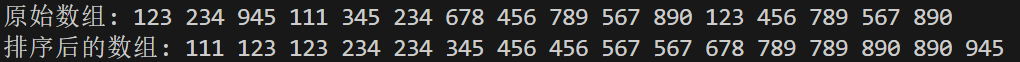
\includegraphics[width=0.95\textwidth]{picture/Screenshot 2024-10-20 162121.png}
    \caption{斐波那契堆排序运行效果}
\end{figure}


\section{任务四:生成测试数据}
\subsection{任务内容}
\begin{itemize}
    \item 编写代码或脚本自动生成测试数据(随机生成浮点数或整数)。
    \item 测试数据应覆盖不同规模的数据集,其中必须包含至少 100 000 条数据的排序任务。
\end{itemize}

\subsection{任务分析}
任务要求编写代码或脚本来自动生成测试数据,这些数据应包括随机生成的浮点数或整数,并且需要覆盖
不同规模的数据集,其中必须包含至少 100,000 条数据的排序任务。这个任务的目的是为了确保排序算法在
不同数据规模下的性能测试具有代表性和全面性,从而能够更准确地评估算法的效率和适用性。

\subsection{任务实现}
\subsubsection{自动生成测试数据}
下面是一个自动生成测试数据的C语言代码,可以自动生成从100到1000000000条测试
数据。
\begin{lstlisting}
    #include <stdio.h>
    #include <stdlib.h>
    #include <time.h>
    
    // 生成随机数据的函数
    void generate_random_data(int size, const char *filename, int data_type) {
        FILE *file = fopen(filename, "w"); // 打开文件以写入数据
        if (file == NULL) {
            perror("Failed to open file"); // 如果文件打开失败,输出错误信息
            exit(EXIT_FAILURE);
        }
    
        for (int i = 0; i < size; i++) {
            if (data_type == 0) {
                // 生成随机浮点数
                float random_float = (float)rand() / RAND_MAX * 2000.0f - 1000.0f;
                fprintf(file, "%f\n", random_float); // 将浮点数写入文件
            } else {
                // 生成随机整数
                int random_int = rand() % 2001 - 1000;
                fprintf(file, "%d\n", random_int); // 将整数写入文件
            }
        }
    
        fclose(file); // 关闭文件
    }
    
    int main() {
        srand(time(NULL)); // 初始化随机数生成器
    
        // 定义不同规模的数据集
        int data_sizes[] = {100, 1000, 10000, 100000, 1000000};
        int data_type = 0; // 0 表示浮点数,1 表示整数
    
        for (int i = 0; i < sizeof(data_sizes) / sizeof(data_sizes[0]); i++) {
            int size = data_sizes[i];
            char filename[256];
            snprintf(filename, sizeof(filename), "random_data_%d.txt", size); // 生成文件名
            generate_random_data(size, filename, data_type); // 生成随机数据并保存到文件
            printf("Generated and saved %d random data points to %s\n", size, filename); // 输出提示信息
        }
    
        return 0;
    }
\end{lstlisting}


\section{任务五:编译与性能测试}
\subsection{任务内容}
\begin{itemize}
    \item 使用不同等级的 gcc 编译优化选项(如 -O0, -O1, -O2, -O3, -Ofast 等)对冒泡排序和堆排序代码进行编译。
    \item 记录各优化等级下的排序算法性能表现(如执行时间和资源占用)。
\end{itemize}

\subsection{任务分析}
任务要求通过使用不同等级的 gcc 编译优化选项(如 -O0, -O1, -O2, -O3, -Ofast)对冒泡
排序和堆排序代码进行编译,并记录各优化等级下的排序算法性能表现(如执行时间和资源占用)。这
程旨在评估编译器优化对算法性能的影响,通过对比不同优化等级下的性能数据,分析编译优化对算法执行
效率的提升效果。

\subsection{任务实现}
为了方便操作,我们使用VSCode来减轻操作负担。
在VSCode中,我们可以很方便地设置编译器的编译选项,然后编译运行程序。
由于任务不多,所以我们手动改变编译选项,然后编译运行程序。
我在程序中加入一些打印语句,以便于观察程序运行时的时间和资源占用。
修改后的代码如下:

\subsubsection{冒泡排序}
\begin{lstlisting}
    #include <stdio.h>
    #include <stdlib.h>
    #include <time.h>
    #include <sys/resource.h> // 添加资源使用库
    
    // 使用冒泡排序算法对数组进行排序
    void bubbleSort(float arr[], int n) {
        int i, j;
        for (i = 0; i < n-1; i++) {
            for (j = 0; j < n-i-1; j++) {
                if (arr[j] > arr[j+1]) {
                    // 交换 arr[j] 和 arr[j+1]
                    float temp = arr[j];
                    arr[j] = arr[j+1];
                    arr[j+1] = temp;
                }
            }
        }
    }
    
    // 打印数组中的元素
    void printArray(float arr[], int size) {
        int i;
        for (i = 0; i < size; i++)
            printf("%f ", arr[i]);
        printf("\n");
    }
    
    // 主函数,程序的入口
    int main() {
        FILE *file;
        char filename[] = "random_data_100000.txt"; // 文件名
        float *arr; // 使用动态内存分配
        int n = 0; // 数组中元素的数量
        clock_t start, end; // 用于记录时间的变量
        double cpu_time_used; // 用于存储执行时间
        struct rusage usage_start, usage_end; // 用于记录资源使用情况
    
        // 打开文件
        file = fopen(filename, "r");
        if (file == NULL) {
            printf("无法打开文件 %s\n", filename);
            return 1;
        }
    
        // 动态分配内存
        arr = (float *)malloc(100000 * sizeof(float));
        if (arr == NULL) {
            printf("内存分配失败\n");
            fclose(file);
            return 1;
        }
    
        // 读取文件中的浮点数
        while (fscanf(file, "%f", &arr[n]) != EOF) {
            n++;
        }
    
        // 关闭文件
        fclose(file);
    
        // 记录开始时间
        start = clock();
    
        // 记录开始时的资源使用情况
        getrusage(RUSAGE_SELF, &usage_start);
    
        // 对数组进行排序
        bubbleSort(arr, n);
    
        // 记录结束时间
        end = clock();
    
        // 记录结束时的资源使用情况
        getrusage(RUSAGE_SELF, &usage_end);
    
        // 计算执行时间
        cpu_time_used = ((double) (end - start)) / CLOCKS_PER_SEC;
    
        // 打印排序后的数组
        printf("Sorted array: \n");
        printArray(arr, n);
    
        // 打印执行时间
        printf("执行时间: %f 秒\n", cpu_time_used);
    
        // 打印资源使用情况
        printf("用户 CPU 时间: %ld.%06ld 秒\n", usage_end.ru_utime.tv_sec - usage_start.ru_utime.tv_sec, usage_end.ru_utime.tv_usec - usage_start.ru_utime.tv_usec);
        printf("系统 CPU 时间: %ld.%06ld 秒\n", usage_end.ru_stime.tv_sec - usage_start.ru_stime.tv_sec, usage_end.ru_stime.tv_usec - usage_start.ru_stime.tv_usec);
        printf("最大驻留集大小: %ld KB\n", usage_end.ru_maxrss - usage_start.ru_maxrss);
        printf("页面错误数: %ld\n", usage_end.ru_majflt - usage_start.ru_majflt);
    
        // 打印内存占用情况
        printf("内存占用: %ld KB\n", usage_end.ru_maxrss);
    
        // 释放内存
        free(arr);
    
        return 0;
    }
\end{lstlisting}

\subsubsection{基础堆排序}
\begin{lstlisting}
    #define _GNU_SOURCE
    #include <stdio.h>
    #include <stdlib.h>
    #include <time.h>
    #include <sys/resource.h>
    
    void swap(float* a, float* b) {
        float temp = *a;
        *a = *b;
        *b = temp;
    }
    
    void heapify(float arr[], int n, int i) {
        int largest = i;
        int left = 2 * i + 1;
        int right = 2 * i + 2;
    
        if (left < n && arr[left] > arr[largest])
            largest = left;
    
        if (right < n && arr[right] > arr[largest])
            largest = right;
    
        if (largest != i) {
            swap(&arr[i], &arr[largest]);
            heapify(arr, n, largest);
        }
    }
    
    void heapSort(float arr[], int n) {
        for (int i = n / 2 - 1; i >= 0; i--)
            heapify(arr, n, i);
    
        for (int i = n - 1; i > 0; i--) {
            swap(&arr[0], &arr[i]);
            heapify(arr, i, 0);
        }
    }
    
    void printArray(float arr[], int size) {
        for (int i = 0; i < size; i++)
            printf("%.2f ", arr[i]);
        printf("\n");
    }
    
    int main() {
        FILE *file;
        char filename[] = "random_data_100000.txt";
        float *arr;
        int n = 0;
        int capacity = 1000000; // 初始容量设置为 1000000
    
        // 动态分配内存
        arr = (float *)malloc(capacity * sizeof(float));
        if (arr == NULL) {
            printf("内存分配失败\n");
            return 1;
        }
    
        // 打开文件
        file = fopen(filename, "r");
        if (file == NULL) {
            printf("无法打开文件 %s\n", filename);
            free(arr);
            return 1;
        }
    
        // 读取文件中的浮点数
        while (fscanf(file, "%f", &arr[n]) != EOF) {
            n++;
            if (n >= capacity) {
                capacity *= 2;
                arr = (float *)realloc(arr, capacity * sizeof(float));
                if (arr == NULL) {
                    printf("内存重新分配失败\n");
                    fclose(file);
                    return 1;
                }
            }
        }
    
        // 关闭文件
        fclose(file);
    
        // 记录开始时间
        clock_t start_time = clock();
    
        // 记录开始时的资源使用情况
        struct rusage start_usage, end_usage;
        getrusage(RUSAGE_SELF, &start_usage);
    
        // 对数组进行排序
        heapSort(arr, n);
    
        // 记录结束时间
        clock_t end_time = clock();
    
        // 记录结束时的资源使用情况
        getrusage(RUSAGE_SELF, &end_usage);
    
        // 计算执行时间
        double time_taken = ((double)(end_time - start_time)) / CLOCKS_PER_SEC;
    
        // 计算资源使用情况
        double user_time = (end_usage.ru_utime.tv_sec - start_usage.ru_utime.tv_sec) +
                           (end_usage.ru_utime.tv_usec - start_usage.ru_utime.tv_usec) / 1e6;
        double system_time = (end_usage.ru_stime.tv_sec - start_usage.ru_stime.tv_sec) +
                             (end_usage.ru_stime.tv_usec - start_usage.ru_stime.tv_usec) / 1e6;
        long max_rss = end_usage.ru_maxrss; // 最大驻留集大小(以KB为单位)
    
        // 打印排序后的数组
        printf("排序后的数组: \n");
        printArray(arr, n);
    
        // 打印执行时间
        printf("执行时间: %f 秒\n", time_taken);
    
        // 打印资源使用情况
        printf("用户时间: %f 秒\n", user_time);
        printf("系统时间: %f 秒\n", system_time);
        printf("最大驻留集大小: %ld KB\n", max_rss);
    
        // 释放内存
        free(arr);
    
        return 0;
    }
\end{lstlisting}

\section{任务六:数据记录与可视化}
\subsection{任务内容}
\begin{itemize}
    \item 收集每个编译等级的运行结果和性能数据。
    \item 分析算法的时间复杂度,并将其与实验数据进行对比。
    \item 将数据记录在 CSV 或其他格式文件中。
    \item 使用 Python、MATLAB 等工具绘制矢量图,展示实验结论。
\end{itemize}

\subsection{任务分析}
第六项任务要求参与者对不同编译优化等级下的冒泡排序和堆排序算法
进行性能测试,记录并分析它们的执行时间和资源占用等性能数据。参
与者需要将这些数据收集并记录在CSV或其他格式的文件中,然后使用
如Python或MATLAB等工具进行数据分析,对比算法的理论时间复杂度与
实际测试数据,最后将分析结果和实验数据以图表形式进行可视化展示
,以直观地呈现不同优化级别对算法性能的影响。

\subsection{任务实现}
\subsubsection{收集运行结果}
根据修改后的代码,我们可以手动收集运行时间和性能数据。
\subsubsection{分析算法的时间复杂度}
冒泡排序:最坏、平均时间复杂度为 $O(n^2)$,最好情况为 $O(n)$。

堆排序:最坏、最好、平均时间复杂度均为 $O(n log n)$。

斐波那契堆:主要用于优化某些操作的时间复杂度,如插入、查找最小元素、合并堆等操作的时间复杂度为 $O(1)$,删除最小元素的时间复杂度为 $O(log n)$。


\subsubsection{记录数据}
数据很少,所以我们手动将数据记录在CSV文件中。

\subsubsection{绘制图表}
我们使用Python,将CSV文件中的数据可视化,绘制图表。

\begin{lstlisting}
    import matplotlib.pyplot as plt
    import numpy as np
    
    # 数据
    sorting_types = ['o0', 'o1', 'o2', 'o3', 'ofast']
    execution_times = [17.560164, 10.706081, 10.475388, 17.650028, 17.333006]
    user_cpu_times = [17.560154, 10.704898, 10.474443, 17.650028, 17.333006]
    system_cpu_times = [0.000010, 0.001183, 0.000946, 0.000000, 0.000000]
    memory_footprints = [2096, 2100, 2100, 2100, 2100]
    
    # 定义颜色
    colors = ['skyblue', 'lightgreen', 'lightcoral', 'lightgrey']
    
    # 绘制条形图
    def plot_bar_chart(data, title, ylabel, color):
        plt.figure(figsize=(10, 6))
        index = np.arange(len(sorting_types))
        plt.bar(index, data, color=color)
        plt.title(title)
        plt.xlabel('Sorting Type')
        plt.ylabel(ylabel)
        plt.xticks(index, sorting_types)
        plt.ylim(0, max(data) * 1.1)  # 设置y轴范围
        for i, value in enumerate(data):
            plt.text(i, value + 0.1, f'{value:.2f}', ha='center', va='bottom')
        plt.savefig(f'{title.lower().replace(" ", "_")}.svg', format='svg')
        plt.show()
    
    # 绘制执行时间图表
    plot_bar_chart(execution_times, 'Execution Time', 'Execution Time (seconds)', colors[0])
    
    # 绘制用户CPU时间图表
    plot_bar_chart(user_cpu_times, 'User CPU Time', 'User CPU Time (seconds)', colors[1])
    
    # 绘制系统CPU时间图表
    plot_bar_chart(system_cpu_times, 'System CPU Time', 'System CPU Time (seconds)', colors[2])
    
    # 绘制内存占用图表
    plot_bar_chart(memory_footprints, 'Memory Footprint', 'Memory Footprint (KB)', colors[3])
\end{lstlisting}

\subsubsection{结果展示}
\begin{figure}[H]
    \centering
    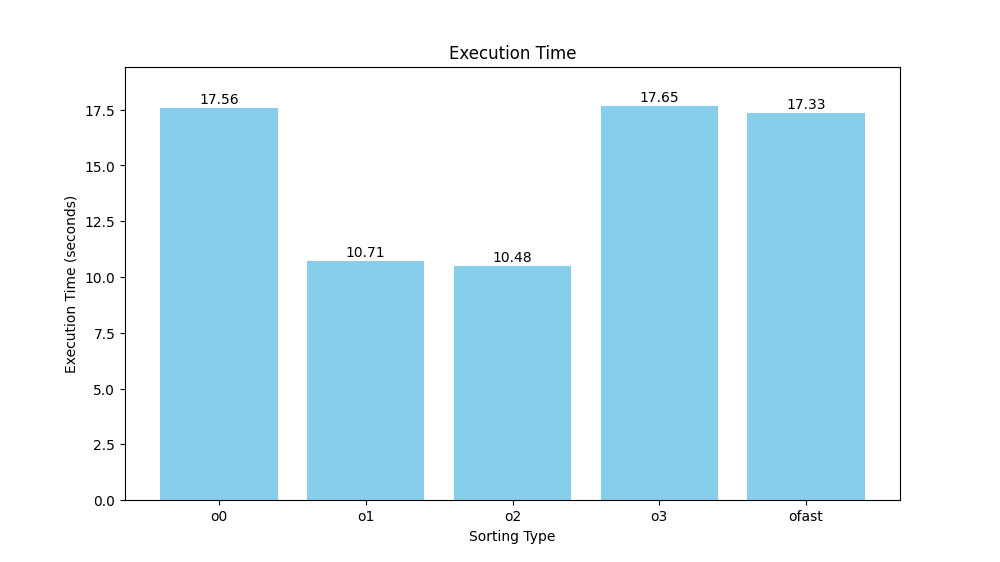
\includegraphics[width=0.8\textwidth]{picture/Figure_1.png}
    \caption{冒泡排序算法执行时间}
\end{figure}

\begin{figure}[H]
    \centering
    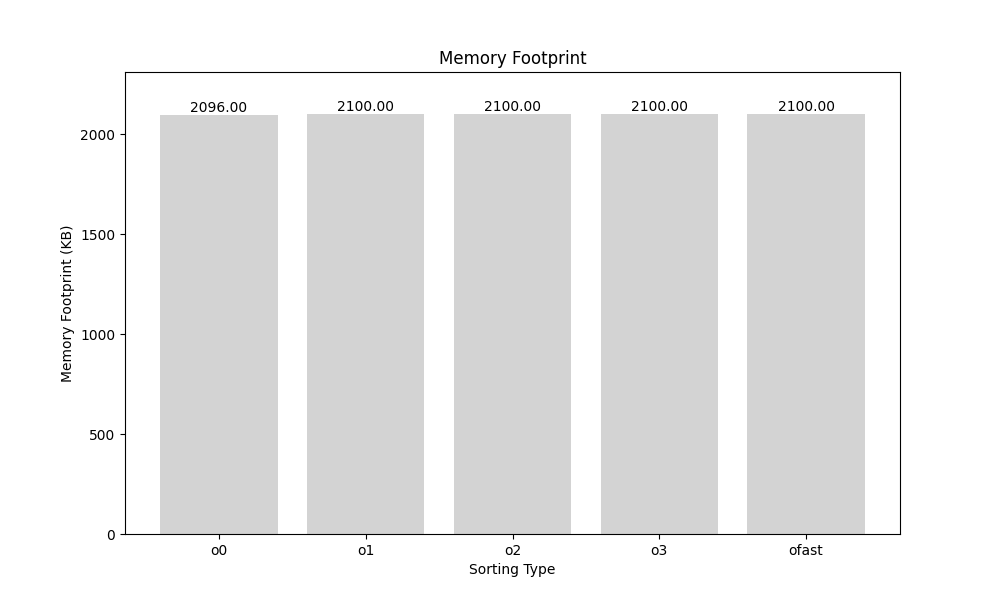
\includegraphics[width=0.8\textwidth]{picture/Figure_2.png}
    \caption{冒泡排序算法内存占用}
\end{figure}

\begin{figure}[H]
    \centering
    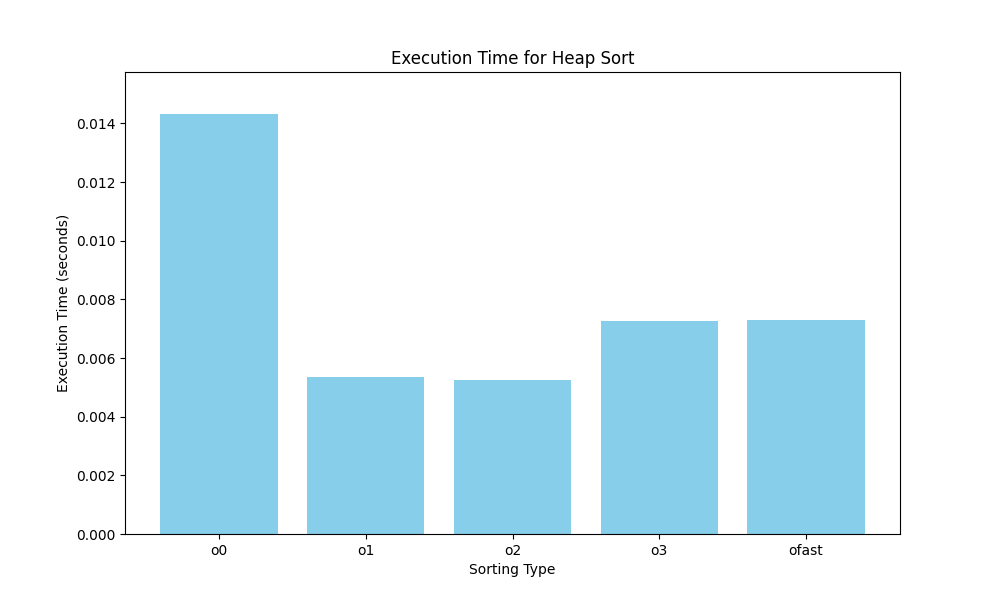
\includegraphics[width=0.8\textwidth]{picture/Figure_3.png}
    \caption{堆排序算法执行时间}
\end{figure}

\begin{figure}[H]
    \centering
    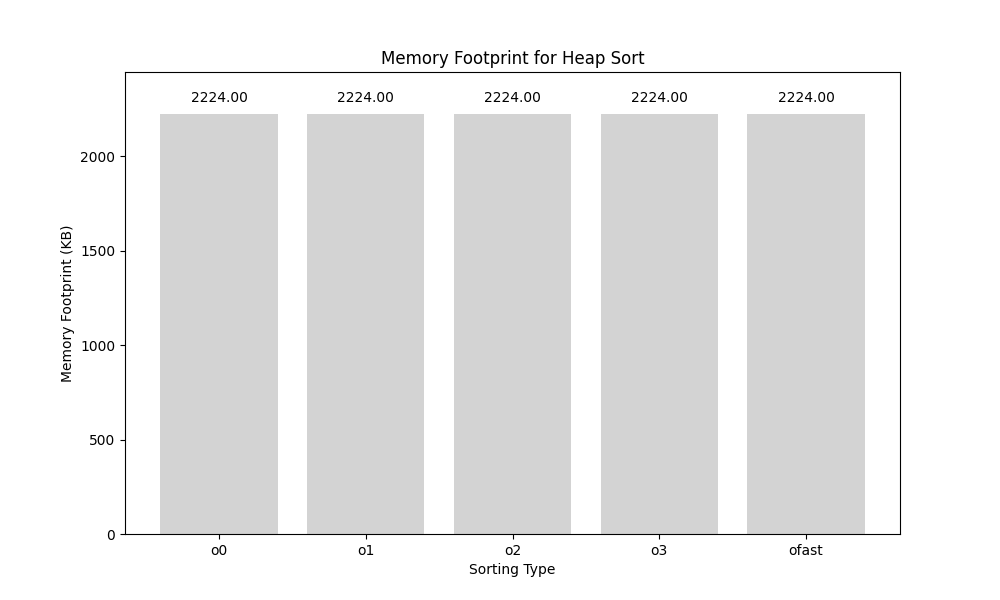
\includegraphics[width=0.8\textwidth]{picture/Figure_4.png}
    \caption{堆排序算法内存占用}
\end{figure}

可以从实验数据看到,对于冒泡排序,o1、o2选项相较于其他选项
明显减少了执行时间,但是内存占用几项基本持平。
对于堆排序,每个优化选项的执行时间都明显减少,但o1、o2选项
相较于o3、ofast选项运行时间更少,内存占用几项基本持平。

不过,由于时间复杂度不同,基础堆排序的执行时间远远少于
冒泡排序,这体现很明显。

\section{实验过程中遇到的问题及解决方案}
实验中最大的问题就是难以解决能力之外的问题,比如斐波那契堆的实
现,虚拟机的配置,以及对未知领域的探索等等。
在这其中,我也积累了很多解决方法,比如:
1:利用AI,AI几乎帮我解决了百分之八十的问题。
2:利用搜索引擎,查找前人的经验,解决问题。
3:从B站、知乎、GitHub等平台学习,找到解决方法。

\end{document}